\documentclass[a4paper,12pt]{report}

%% packages :
% Packages :
\usepackage[indonesian]{babel}
\usepackage[T1]{fontenc}
\usepackage[utf8]{inputenc}
\usepackage{listings}
\usepackage{amssymb}
\usepackage{amsmath}
\usepackage{amsfonts}
\usepackage{graphicx,marvosym}
\usepackage{sidecap}
\usepackage{wrapfig}
\usepackage{enumitem}
\usepackage{parskip}
\usepackage[usenames, dvipsnames]{color}
\usepackage{fancyhdr} % For Page Style.
\usepackage{hyperref}
\usepackage{import}
\usepackage{bookmark} % For Bookmark
\usepackage{setspace}
\usepackage{sectsty}
\usepackage{float}
\usepackage{geometry}
\usepackage{babel}
\usepackage{calc, blindtext}
\usepackage[svgnames]{xcolor} % Required to specify font color
\usepackage{titlesec} % Title Section Settings
\usepackage{tocloft}
\usepackage{titling}
\usepackage{multicol}
%Options: Sonny, Lenny, Glenn, Conny, Rejne, Bjarne, Bjornstrup
%\usepackage[Glenn]{fncychap}
\usepackage{graphicx} % Required for box manipulation
\usepackage[font=scriptsize]{caption} % For Image Caption

% Font Package :
\usepackage{lmodern} % Latin Modern Sans Serif
\usepackage{tgtermes} % Gyre Termes
\usepackage{tgpagella} % Gyre Pagella
\usepackage{tgbonum} % Gyre Bonum
\usepackage{tgschola} % Gyre Schola
\usepackage{times} % Times
\usepackage{utopia} % Utopia / Fourier
\usepackage{palatino} % Palatino
\usepackage{bookman} % Bookman
\usepackage{charter} % Charter
\usepackage{tgadventor} % Tex Gyre Adventor
\usepackage{tgheros} % Tex Gyre Heros
\usepackage{helvet} % Helvetica
\usepackage{tgcursor} % Gyre Cursor
\usepackage{courier} % Courier

%% Macros Helper :
\newcommand{\latex}{\LaTeX\xspace}

%\renewcommand{\rmdefault}{phv} % Arial
%\renewcommand{\sfdefault}{phv} % Arial
\renewcommand\thepart{\arabic{part}}
\renewcommand\cftpartpresnum{Part~}

\newcommand\solidrule[1][1cm]{\rule[0.5ex]{#1}{.4pt}}
\newcommand\dashedrule{\mbox{%
		\solidrule[2mm]\hspace{2mm}\solidrule[2mm]\hspace{2mm}\solidrule[2mm]}}

\def\magicref#1{\expandafter\magicref@i#1\@nil}
\def\magicref@i#1::#2\@nil{section \ref{#1} on page \pageref{#1::#2}}
\makeatother

\newcommand{\Twomin}[1]{-\hspace{0.5mm}-#1}

%% Layout Settings :
%% Hyperlink Setup :
\hypersetup{
	colorlinks,
	citecolor=black,
	filecolor=black,
	linkcolor=black,
	urlcolor=black
}

%% Font Setting :
%\renewcommand{\rmdefault}{lmr}
\renewcommand{\familydefault}{lmr}
\renewcommand{\sfdefault}{phv}

%% Format Section
\sectionfont{\fontfamily{qhv}\fontseries{b}\selectfont}
\fontfamily{lmr}
\titlespacing{\section}{0pt}{10pt}{0pt}
\titlespacing{\subsection}{0pt}{10pt}{0pt}
\titlespacing{\subsubsection}{0pt}{5pt}{0pt}
\setcounter{secnumdepth}{5}   
\setcounter{tocdepth}{5}

%% Caption Figure Setting :
\DeclareCaptionFormat{tfigureFormat}{#1#2#3\vspace{3pt}}
\DeclareCaptionFormat{bfigureFormat}{\hrulefill\par\medskip#1#2#3}
\captionsetup[figure]{font=scriptsize,labelfont={sf},textfont={sf,bf},format=tfigureFormat}

% Color
\definecolor{mygray}{gray}{0.6}
\definecolor{backcolour}{rgb}{0.95,0.95,0.92}

%% Layout for Title Pages :
% macros for title page :
\newcommand*{\plogo}{\fbox{$\mathcal{OI}$}} % Generic publisher logo
\newcommand*{\rotrt}[1]{\rotatebox{90}{#1}} % Command to rotate right 90 degrees
\newcommand*{\rotlft}[1]{\rotatebox{-90}{#1}} % Command to rotate left 90 degrees
\newcommand*{\titleBC}{\begingroup % Create the command for including the title page in the document


\endgroup}

%% Hyphenation Settings :
\hyphenation{cryp-to-graphy}
\hyphenation{Bene-dict}
\hyphenation{Li-nux}
\hyphenation{li-nux}
\hyphenation{ke-stabilan}
\hyphenation{saja}
\hyphenation{saat}
\hyphenation{kali}
\hyphenation{berikut}
\hyphenation{ilmu}
\hyphenation{mendapat-kan}
\hyphenation{akan}
\hyphenation{ser-ver}
\hyphenation{soft-ware}
\hyphenation{Debi-an}
\hyphenation{debi-an}
\hyphenation{dengan}
\hyphenation{di-dirikan}
\hyphenation{pada}
\hyphenation{installer}
\hyphenation{anaconda}
\hyphenation{Anaconda}
\hyphenation{perangkat}
\hyphenation{mig-rasi}
\hyphenation{makas}
\hyphenation{Anda}
\hyphenation{hard}
\hyphenation{kemudian}
\hyphenation{tahu}
\hyphenation{memper-baiki}
\hyphenation{Adminis-trator}
\hyphenation{banyak}
\hyphenation{baik}
\hyphenation{meng-harapkan}
\hyphenation{License}
\hyphenation{mengantar}
\hyphenation{IRGSH}
\hyphenation{sing-kronisasi}
\hyphenation{sing-kroni-sasi}
\hyphenation{BlankOn-Dev}
\hyphenation{BlankOn}
\hyphenation{dependensi}
\hyphenation{di-guna-kan}
\hyphenation{down-load}
\hyphenation{lebih}
\hyphenation{lainnya}

%% Listing code Languages Settings :

\lstdefinelanguage{Ini}
{
	basicstyle=\ttfamily\scriptsize,
	columns=fullflexible,
	backgroundcolor=\color{backcolour},
	morecomment=[s][\color{Orchid}\bfseries]{[}{]},
	morecomment=[l]{\#},
	morecomment=[l]{;},
	commentstyle=\color{gray}\ttfamily,
	morekeywords={},
	keywordstyle={\color{green}\bfseries}
}

\lstdefinelanguage{ShellBash}
{
	basicstyle=\color{blue}\ttfamily\footnotesize,
	columns=fullflexible,
	backgroundcolor=\color{backcolour},
	morecomment=[s][\color{Orchid}\bfseries]{[}{]},
	morecomment=[l]{\#},
	morecomment=[l]{;},
	commentstyle=\color{gray}\ttfamily,
	morekeywords={},
}
\lstdefinelanguage{ShellBash2}
{
	basicstyle=\color{blue}\ttfamily\scriptsize,
	columns=fullflexible,
	backgroundcolor=\color{backcolour},
	morecomment=[s][\color{Orchid}\bfseries]{[}{]},
	morecomment=[l]{\#},
	morecomment=[l]{;},
	commentstyle=\color{gray}\ttfamily,
	morekeywords={
		boidev
		},
}
\lstdefinelanguage{ShellBash3}
{
	basicstyle=\color{Black}\ttfamily\scriptsize,
	columns=fullflexible,
	backgroundcolor=\color{backcolour},
	morecomment=[s][\color{Violet}\bfseries]{[}{]},
	morecomment=[l]{\#},
	morecomment=[l]{;},
	commentstyle=\color{gray}\ttfamily,
	keywordstyle=\color{gray}\ttfamily,
	morekeywords={},
}

\lstdefinestyle{myCustomMatlabStyle}{
	columns=fullflexible,
	tabsize=4,
	showspaces=false,
	showstringspaces=false,
	breaklines=true,
	basicstyle=\color{blue}\scriptsize\ttfamily,
	stringstyle=\color{red}\ttfamily,
	morecomment=[s][\color{Orchid}\bfseries]{[}{]},
	morecomment=[l]{\#},
	morecomment=[l]{;},
	commentstyle=\color{Gray}\ttfamily
}
\lstset{style=myCustomMatlabStyle}
\lstset{framextopmargin=50pt}
\graphicspath{{img/}}

\begin{document}
	\pagenumbering{roman}

	%% Cover
	\pagestyle{empty}
	\begin{titlepage}

\addcontentsline{toc}{chapter}{Cover}

%	\titleBC % This command includes the title page
\centering % Center all text
\def\CP{\textit{\Huge BlankOnDev v0.1005}} % Title

\settowidth{\unitlength}{\CP} % Set the width of the curly brackets to the width of the title
{\color{LightGoldenrod}\resizebox*{\unitlength}{\baselineskip}{\rotrt{$\}$}}} \\[\baselineskip] % Print top curly bracket
\textcolor{Sienna}{\CP} \\[\baselineskip] % Print title
{\color{RosyBrown}\Large User Guide} \\ % Tagline or further description
{\color{LightGoldenrod}\resizebox*{\unitlength}{\baselineskip}{\rotlft{$\}$}}} % Print bottom curly bracket

\vfill % Whitespace between the author name and the publisher logo

\begin{center}
	
\includegraphics[height=2cm]{logo.png}\\
\end{center}

\vfill % Whitespace between the title and the author name
\textbf{Author:}\\
\vspace{5mm}
{\Large\textbf{Achmad Yusri Afandi}}\\ % Author name
\vspace{5mm}
{\Large\textbf{BlankOn Developer Team}}\\ % Author name

\vfill % Whitespace between the author name and the publisher logo


2017 % Year published
\end{titlepage}

\title{Tutorial BlankOnDev version 0.1005}
\author{Achmad Yusri Afandi \\ and \\ BlankOn Develper Team}
\date{\today}
	\clearpage

	%% Table of Content :
	\pagestyle{fancy}
	\fancyhf{}
	\fancyhead[LE]{\thepage}
	\fancyhead[RO]{\thepage}
	\fancyhead[RE]{\nouppercase{\textbf{\leftmark}}}
	\fancyhead[LO]{\textbf{Tutorial BlankOnDev version 0.1005}}
	\setlength{\parindent}{1cm}
	\setlength{\parskip}{0.25cm}
	\phantomsection
	\tableofcontents
	\addcontentsline{toc}{chapter}{Daftar Isi}
	\clearpage
%	\SetWatermarkText{
\includegraphics[width=9cm]{logo.png}}
	%% Bab 1 - Pengenalan
	%% For Page Style :
\pagestyle{fancy}
\fancyhf{}
\fancyhead[LE]{\thepage}
\fancyhead[RO]{\thepage}
\fancyhead[RE]{\nouppercase{\textbf{\leftmark}}}
\fancyhead[LO]{\textbf{Tutorial BlankOnDev version 0.1005}}
\setlength{\parindent}{1cm}
\setlength{\parskip}{0.25cm}

%% Format Chapter
\definecolor{RoyalRed}{RGB}{157,16, 45}
\chapterfont{\fontfamily{bch}\fontseries{b}\selectfont}

\titleformat{\chapter}[display]
{\normalfont\bfseries\filcenter}
{\LARGE}
{1ex}
{\titlerule[2pt]
	\textbf{{\LARGE \thechapter} \hspace{1mm}\textbf{{\LARGE |}}}
	\hspace{1mm}%
	\LARGE}
[\vspace{1ex}%
{\titlerule[2pt]}]

\chapter{Pengenalan}

%% Page Numbering for chapter :
\pagenumbering{arabic}

\section{Apa itu BlankOnDev ?}\label{sec:what_blankondev}
\noindent
\textbf{BlankOnDev} merupakan Tools untuk melakukan aktifitas sebagai pengembang GNU/Linux BlankOn.
Terdapat beberapa pekerjaan sebagai pengembang BlankOn khususnya untuk \textbf{Tim Pemaket} yang dilakukan dengan cara manual menggunakan beberapa perintah Linux, yang menurut penulis cukup tradisional.

\noindent
Pada tools \textbf{BlankOnDev} \textit{rencana} akan memiliki beberapa fitur untuk mempermudah pekerjaan Tim Pemaket meliputi :
\begin{enumerate}
	\item Manajemen pengaturan repositori pada Sistem Linux Pemaket
	
	\item Persiapan Sistem Linux Pemaket sebelum melakukan aktifitas pemaket.
	
	\item System manajemen builder Paket dari Source menjadi file \textbf{.deb} yang siap untuk di install dengan perintah \texttt{dpkg -i <file\_packages.deb>}.
	
	\item Melakukan patching atau perbaikan bugs yang terpadat pada paket-paket tertentu.
	
	\item Membuat format paket debian yang nantinya akan diteruskan ke server \textbf{irgsh}\footnote{\textbf{irgsh} merupakan mesin builder paket BlankOn GNU/Linux} untuk dilakukan proses build source menjadi paket debian yaitu file \textbf{.deb}, yang kemudian akan di dorong ke \textbf{reprepo}\footnote{\textbf{reprepo} merupakan tool untuk menangani local repositori}.
	
	\item Migrasi data paket debian yang sebelumnya tersimpan dalam server bazaar repository ke server github repository.
	
	\item Sistem pembuatan Repositori mirror secara otomatis dengan sistem singkronisasi yang tercontrol.
\end{enumerate}

\noindent
Fitur \textbf{BlankOnDev v0.1005} yang sudah rampung dan siap untuk digunakan :
\begin{itemize}
	\item Fitur Migrasi data paket debian yang sebelumnya tersimpan pada server bazaar ke server github repository.
\end{itemize}

\section{Mengapa BlankOnDev Harus dibuat ?}\label{sec:why}
\noindent
Ada beberapa aktifitas yang mememakan banyak waktu jika harus dilakukan dengan cara tradisional di Sistem Operasi GNU/Linux. GNU/Linux BlankOn merupakan Distribusi Linux turunan Debian GNU/Linux, dengan basis Debian GNU/Linux sebenarnya sudah memberikan banyak kemudahan dalam penggunaannya, akan tetapi tetap memakan waktu yang banyak. Sedangkan ada hal yang lebih penting daripada sekedar menjalankan perintah linux satu per satu yaitu Kestabilan dari Distribusi Sistem Operasi GNU/Linux. 

\noindent
Berikut beberapa kasus yang menginspirasi penulis untuk membuat Tools dengan nama \textbf{BlankOnDev}, yaitu :
\begin{itemize}
	\item Konfigurasi sistem lokal pemaket sebelum melakukan aktifitas pemaket, ini juga harus dilakukan banyak percobaan untuk menghasilkan konfigurasi yang stabil.
	
	\item Sistem kontrol server repositori yang menurut penulis masih perlu diperbaiki untuk mencegah terjadi permasalahan di server repositori GNU/Linux BlankOn. Dan ketika terjadi permasalahan dapat diselesaikan dalam kurung waktu sangat singkat.
	
	\item Build Paket di mesin lokal Pemaket. Aktifitas ini, juga bisa dikatakan sangat panjang jika terjadi permasalahan seperti patch bugs paket BlankOn. Aktifitas build tanpa adanya permasalahan juga akna sangat panjang, jika Pemaket harus menentukan versi paket yang akan dipaketkan atau melakukan uji coba terhadap versi paket sebelum di dorong ke \textbf{irgsh}.
	
	\item Build paket beserta dependensi paket. Setiap paket utama yang akan dibuild tentunya memiliki dependensi atau dalam artian adanya keterkaitan antar paket lainnya. Agar paket utama yang dibuild dapat stabil saat installasi maupun penggunaannya, maka dependensi paket juga harus sama stabilnya. Kemudian, jika hal ini dilakukan secara manual oleh pemaket, maka pasti akan memakan banyak waktu. (Lihat \hyperref[text:apt-rdepends]{\textbf{apt-rdepends}})
	
	\item Pengaturan repositori di sistem pemaket, proses penggantian alamat Repositori masih tergolong manual, karena harus mengedit file konfigurasi di \texttt{/etc/apt/sources.list}. Jika hanya sebagai pengguna biasa ini tidak masalah. Namun untuk pengembang ini sangat banyak makan waktu ketika harus melakukan pengujian terhadap repositori.
	
	\item Proses pencarian source sebelum build paket. Ini juga akan memakan banyak waktu untuk mencari source paket yang sesuai dari beberapa repositori Debian GNU/Linux maupun turunannya.
\end{itemize}

\noindent
Selain butir-butir diatas penulis juga terinspirasi dengan \textbf{Debian Manifasto} yang di tulis oleh \textit{Ian A. Murdock}, sebagai konstruksi awal dari pengembangan Debian GNU/Linux. Dan juga menjadi landasan pengembangan \textit{BlankOnDev Tools}. (Lihat \hyperref[appdx::deb_manifesto]{\textbf{Debian Manifesto}} di \textit{Halaman \pageref{appdx::deb_manifesto}})

\section{Teknologi yang digunakan oleh BlankOnDev}\label{sec:tekno}
\noindent
Pengembangan \textit{BlankOnDev tools} menggunakan bahasa pemrogram \textbf{Perl} demi kemudahan penulis untuk membuat beberapa tools, apalagi Perl sangat powerful untuk pemrograman text. 

\noindent
Terdapat beberapa paket-paket Debian yang masih menggunakan \textit{Perl} sampai saat ini, seperti beberapa tools \textit{dpkg}, \textit{apt} dan masih banyak lagi tool-tool yang selama ini sering digunakan dan dibuat dengan bahasa pemrograman \textbf{Perl}. 

\noindent
\textit{Perl philosophy : "Kami dapat mengajari Anda bagaimana kami melukis, tapi kami tidak dapat mengajari Anda bagaimana Anda melukis"}

\noindent
Prototype \textbf{apt-get} dan \textbf{aptitude} juga awalanya menggunakan bahasa pemrogram Perl yang kemudian ditulis ulang ke C/C++. Tools \textbf{tasksel} yang berjalan pada instalasi mode text Debian GNU/Linux dan juga bisa dijalakan setelah instalasi, masih menggunakan Perl. Beberapa hal ini juga menjadi alasan penulis untuk membuat program BlankOnDev dengan bahasa pemrogram perl. Konsep seperti tool \textbf{tasksel} yang akan digunakan oleh penulis kedepannya untuk memenuhi seluruh daftar fitur yang disebutkan pada \textit{Tutorial} ini.

\noindent
Salah satu tools Debian yang digunakan untuk melihat semua dependensi terhadap suatu paket tertentu yaitu \textbf{apt-rdepends}. output dari tools dari \texttt{apt-rdepends} seperti berikut :\label{text:apt-rdepends}
\pagebreak
\begin{lstlisting}[language=ShellBash]
$ apt-rdepends tar
Reading package lists... Done
Building dependency tree       
Reading state information... Done
tar
	PreDepends: libacl1 (>= 2.2.51-8)
	PreDepends: libc6 (>= 2.17)
	PreDepends: libselinux1 (>= 1.32)
libacl1
	Depends: libattr1 (>= 1:2.4.46-8)
	Depends: libc6 (>= 2.14)
	PreDepends: multiarch-support
libattr1
	Depends: libc6 (>= 2.4)
	PreDepends: multiarch-support
libc6
	Depends: libgcc1
libgcc1
	Depends: gcc-4.9-base (= 4.9.2-10)
	Depends: libc6 (>= 2.14)
	PreDepends: multiarch-support
gcc-4.9-base
multiarch-support
	Depends: libc6 (>= 2.3.6-2)
libselinux1
	Depends: libc6 (>= 2.14)
	Depends: libpcre3 (>= 8.10)
	PreDepends: multiarch-support
libpcre3
	Depends: libc6 (>= 2.14)
	PreDepends: multiarch-support
\end{lstlisting}

\noindent
Tool \texttt{apt-rdepends} juga merupakan tools yang sangat memudahkan dalam pencarian dependensi suatu paket tertentu. Tool ini juga akan menjadi sumber informasi untuk pembuatan fitur Build paket di program \textbf{BlankOnDev}.

\section{List Command}
\noindent
Daftar perintah pada program \textbf{BlankOnDev} terdiri dari 2 bagian yaitu :
\begin{itemize}
	\item Perintah untuk konfigurasi program
	\item Perintah untuk Migrasi Paket.
\end{itemize}

\subsection{Perintah Konfigurasi Program}
\noindent
Bagian ini terdiri dari 10 Perintah yaitu :
\begin{enumerate}
	\item Perintah \texttt{\textbf{boidev config}} - Perintah ini digunakan untuk melakukan pengaturan sebelum penggunaan program lebih lanjut.
	
	\item Perintah \texttt{\textbf{boidev mig\_prepare}} - Perintah ini digunakan persiapan sebelum melakukan migrasi paket, seperti \textbf{url branch}, \textbf{url github}, \textbf{email github}, dan data untuk proses Generate key dengan \textbf{GnuPG}.
	
	\item Perintah \texttt{\textbf{boidev install-pkg}} - Perintah ini digunakan untuk instalasi beberapa paket debian yang dibutuhkan untuk Tim Pemaket.
	
	\item Perintah \texttt{\textbf{boidev gpg-auth}} dan \texttt{\textbf{boidev gpg-auth-dec}} - Perintah ini digunakan untuk melihat \textbf{nama}, \textbf{email} dan \textbf{passphrase} \textbf{GnuPG} yang digunakan untuk \textit{Generate Key}.
	
	\item Perintah \texttt{\textbf{boidev gpg-genkey}} - Perintah ini digunakan untuk melakukan \textit{Generate key GnuPG}
	
	\item Perintah \texttt{\textbf{boidev list-cfg}} - Perintah ini digunakan untuk melihat daftar konfigurasi program \textbf{BlankOnDev} yang telah dilakukan.
	
	\item Perintah \texttt{\textbf{boidev list-file}} - Perintah ini digunakan untuk melihat daftar file konfigurasi yang tersimpan pada sistem program \textbf{BlankOnDev}.
	
	\item Perintah \texttt{\textbf{boidev rilis}} - Perintah Ini digunakan untuk mengubah rilis \textbf{BlankOn} yang digunakan pada program \textbf{BlankOnDev}
	
	\item Perintah \texttt{\textbf{boidev -v}} atau \texttt{\textbf{boidev \Twomin{version}}} - Perintah ini digunakan untuk melihat versi tools \textbf{BlankOnDev}
\end{enumerate}

\subsection{Perintah Migrasi Paket}
\noindent
Bagian ini terdiri dari 17 Perintah yaitu :
\begin{enumerate}
	\item Perintah \texttt{\textbf{boidev bzr2git}} - Perintah ini merupakan perintah yang digunakan untuk melakukan Migrasi paket dari repositori \textbf{Bazaar} ke repositori \textbf{Github}
	
	\item Perintah \texttt{\textbf{boidev bzr2git addpkg-group}} - Perintah ini merupakan perintah yang digunakan untuk menambahkan group paket yang akan dimigrasi.

	\item Perintah \texttt{\textbf{boidev bzr2git addpkg}} - Perintah ini merupakan perintah yang digunakan untuk menambahkan nama paket yang akan di migrasi

	\item Perintah \texttt{\textbf{boidev bzr2git addpkg-file}} - Perintah ini merupakan perintah yang digunakan untuk menambahkan nama paket yang akan dimigrasi melalui file list paket yang berekstensi \textbf{.boikg}

	\item Perintah \texttt{\textbf{boidev bzr2git remove-pkg-group}} - Perintah ini merupakan perintah yang digunakan untuk menghapus nama group paket migrasi. Perintah ini akan menghapus semau daftar paket yang terkait dengan \textbf{Group}.

	\item Perintah \texttt{\textbf{boidev bzr2git rename-pkg-group}} - Perintah ini merupakan perintah yang digunakan untuk mengubah nama group paket migrasi.

	\item Perintah \texttt{\textbf{boidev bzr2git remove-pkg}} - Perintah ini merupakan perintah yang digunakan untuk menghapus nama paket yang terdaftar pada system program \textbf{BlankOnDev}

	\item Perintah \texttt{\textbf{boidev bzr2git list-pkg}} - Perintah ini merupakan perintah yang digunakan untuk melihat daftar paket yang terdaftar pada system program \textbf{BlankOnDev}.

	\item Perintah \texttt{\textbf{boidev bzr2git list-pkg-group}} - Perintah ini merupakan perintah yang digunakan untuk melihat daftar group paket.

	\item Perintah \texttt{\textbf{boidev bzr2git search-pkg}} - Perintah ini merupakan perintah yang digunakan utnuk mencari nama paket yang terdaftar pada system program \textbf{BlankOnDev}.

	\item Perintah \texttt{\textbf{boidev bzr2git branch}} - Perintah ini merupakan perintah yang digunakan untuk mengambil/download paket dari repositori bazaar berdasarkan nama paket yang sudah terdaftar pada system program \textbf{BlankOnDev}.

	\item Perintah \texttt{\textbf{boidev bzr2git bzr-cgit}} - Perintah ini merupakan perintah yang digunakan untuk mengkonversi format repositori bazaar ke format repositori github, berdasarkan nama paket yang sudah terdaftar pada system program \textbf{BlankOnDev}

	\item Perintah \texttt{\textbf{boidev bzr2git git-push}} - Perintah ini merupakan perintah yang digunakan untuk mendorong/upload yang sudah didownload, berdasarkan nama paket yang sudah terdaftar pada system program \textbf{BlankOnDev}

	\item Perintah \texttt{\textbf{boidev bzr2git git-push-new}} - Perintah ini merupakan perintah yang digunakan untuk mendorong/upload yang sudah didownload namum belum dikonversi ke format repositori github, berdasarkan nama paket yang sudah terdaftar pada system program \textbf{BlankOnDev}. Perintah ini sama seperti instruksi dari github setelah nama repositori baru ditambahkan.

	\item Perintah \texttt{\textbf{boidev bzr2git git-check}} - Perintah ini merupakan perintah yang digunakan untuk validasi repositori yang sudah diupload ke github.

	\item Perintah \texttt{\textbf{boidev bzr2git re-branch}} - Perintah ini merupakan perintah untuk download ulang paket dari bazaar repositori.

	\item Perintah \texttt{\textbf{boidev bzr2git re-gitpush}} - Perintah ini digunakan untuk memperbaiki kesalahan upload paket ke github yang tidak dilakukan convert format sebelumnya.
\end{enumerate}

\subsection{Perintah help}
\noindent
Bagian ini terdiri dari 17 Perintah yaitu :
\begin{enumerate}
	\item Perintah \texttt{\textbf{boidev help}} - Untuk melihat seluruh help perintah \texttt{boidev}
	
	\item Perintah \texttt{\textbf{boidev bzr2git help}} - Untuk melihat seluruh perintah \texttt{boidev bzr2git}
	
	Adapun perintah help untuk perintah yang diawali dengan perintah \texttt{boidev bzr2git} yaitu :
	\begin{enumerate}
        \item perintah \texttt{\textbf{boidev bzr2git addpkg-group help}}
        \item perintah \texttt{\textbf{bzr2git addpkg help}}
        \item perintah \texttt{\textbf{bzr2git addpkg-file help}}
        \item perintah \texttt{\textbf{bzr2git list-pkg help}}
        \item perintah \texttt{\textbf{bzr2git rename-pkg-group help}}
        \item perintah \texttt{\textbf{bzr2git remove-pkg-group help}}
        \item perintah \texttt{\textbf{bzr2git remove-pkg help}}
        \item perintah \texttt{\textbf{bzr2git search-pkg help}}
        \item perintah \texttt{\textbf{bzr2git branch help}}
        \item perintah \texttt{\textbf{bzr2git bzr-cgit help}}
        \item perintah \texttt{\textbf{bzr2git git-push help}}
        \item perintah \texttt{\textbf{bzr2git git-push-new help}}
        \item perintah \texttt{\textbf{bzr2git git-check help}}
        \item perintah \texttt{\textbf{bzr2git re-branch help}}
        \item perintah \texttt{\textbf{bzr2git re-gitpush help}}
	\end{enumerate}
\end{enumerate}

	%% Bab 2 - Fungsi Command "boidev"
	%% For Page Style :
\pagestyle{fancy}
\fancyhf{}
\fancyhead[LE]{\thepage}
\fancyhead[RO]{\thepage}
\fancyhead[RE]{\nouppercase{\textbf{\leftmark}}}
\fancyhead[LO]{\textbf{Tutorial BlankOnDev version 0.1005}}
\setlength{\parindent}{1cm}
\setlength{\parskip}{0.25cm}
%\fontsize{\normalsize}{baselineskip}

%% Format Chapter
\definecolor{RoyalRed}{RGB}{157,16, 45}
\chapterfont{\fontfamily{bch}\fontseries{b}\selectfont}

\titleformat{\chapter}[display]
{\normalfont\bfseries\filcenter}
{\LARGE}
{1ex}
{\titlerule[2pt]
	\textbf{{\LARGE \thechapter} \hspace{1mm}\textbf{{\LARGE |}}}
	\hspace{1mm}%
	\LARGE}
[\vspace{1ex}%
{\titlerule[2pt]}]
\hyphenation{setelah}

\chapter{Persiapan dan Implementasi}
\label{chap:prepare_impl}

%% Page Numbering for chapter :
\pagenumbering{arabic}
\section{Persiapan}
\label{persiapan}

\noindent
Pada bagian ini akan dijelaskan hal-hal yang perlu dipersipakan sebelum menggunakan program \textbf{BlankOnDev} yaitu "\textbf{rng-tools}".

\subsection{Install dan Konfigurasi \textit{rng-tools}}
\noindent
Untuk install \textbf{rng-tools} dengan perintah

\begin{lstlisting}[language=ShellBash]
sudo apt-get install rng-tools
\end{lstlisting}

\noindent
Kemudian edit file \texttt{/etc/default/rng-tools} dengan perintah :

\begin{lstlisting}[language=ShellBash]
sudo vim /etc/default/rng-tools
\end{lstlisting}

\noindent
Dan tambahkan script \texttt{HRNGDEVICE=/dev/urandom} seperti berikut :

\begin{lstlisting}[language=Ini]
# Configuration for the rng-tools initscript
# $Id: rng-tools.default,v 1.1.2.5 2008-06-10 19:51:37 hmh Exp $

# This is a POSIX shell fragment

# Set to the input source for random data, leave undefined
# for the initscript to attempt auto-detection.  Set to /dev/null
# for the viapadlock driver.
#HRNGDEVICE=/dev/hwrng
#HRNGDEVICE=/dev/null
HRNGDEVICE=/dev/urandom

# Additional options to send to rngd. See the rngd(8) manpage for
# more information.  Do not specify -r/--rng-device here, use
# HRNGDEVICE for that instead.
#RNGDOPTIONS="--hrng=intelfwh --fill-watermark=90% --feed-interval=1"
#RNGDOPTIONS="--hrng=viakernel --fill-watermark=90% --feed-interval=1"
#RNGDOPTIONS="--hrng=viapadlock --fill-watermark=90% --feed-interval=1"
\end{lstlisting}

\noindent
Pada file tersebut hanya menambahkan script \texttt{HRNGDEVICE=/dev/urandom} setelah 
komentar \texttt{\#HRNGDEVICE=/dev/null}.

\noindent
Kemudian, Simpan file dan start service \textbf{rng-tools} seperti contoh perintah berikut:

\begin{lstlisting}[language=ShellBash]
sudo /etc/init.d/rng-tools start
\end{lstlisting}

\subsection{Membuat \textit{SSH Public key authentication} for Github}
\noindent
\normalsize
Konfigurasi ini bertujuan agar pada saat push repositori ke Github tidak lagi harus memasukkan \texttt{Username} dan \texttt{Password} saat proses push repositori.

\subsubsection{Membuat Public key SSH}
\noindent
Jalankan perintah \texttt{\textbf{ssh-keygen -t rsa}} seperti berikut :

\begin{lstlisting}[language=ShellBash]
$ ssh-keygen -t rsa -b 4096 -C "linuxer08@gmail.com"
Generating public/private rsa key pair.
Enter file in which to save the key (/home/yusrideb/.ssh/id_rsa): 
Created directory '/home/yusrideb/.ssh'.

\end{lstlisting}
\noindent
Langsung Saja Tekan Enter pada Kedua form ini.

\begin{lstlisting}[language=ShellBash]
Enter passphrase (empty for no passphrase):
Enter same passphrase again: 
\end{lstlisting}
\begin{lstlisting}[language=ShellBash]
Your identification has been saved in /home/yusrideb/.ssh/id_rsa.
Your public key has been saved in /home/yusrideb/.ssh/id_rsa.pub.
The key fingerprint is:
SHA256:KkcuVZ/vd9mbbtU0w62ThEqa/63ZrdV762h9SIfeRys linuxer08@gmail.com
The key's randomart image is:
+---[RSA 2048]----+
|                 |
|                 |
|        .    .. .|
|       . .... .+o|
|      o S+o. . =+|
|     + .o ..  * *|
|    o +  .  .o.*B|
|     +    .. E=BX|
|           .*+OXB|
+----[SHA256]-----+
\end{lstlisting}

\pagebreak
\subsubsection{Menambahkan SSH Key di Akun Github}

\begin{multicols}{2}
[
\noindent
Pada bagian ini sebagai contoh file \textit{Public Key SSH} berada di\\ \texttt{/home/yusrideb/.ssh/id\_rsa.pub}\\
Setelah itu, masuk ke akun github dan lakukan pengaturan di bagian \textit{SSH and GPG Keys} untuk menanbahkan \textit{SSH Key} pada \textbf{Github} dengan isi dari file\\ \texttt{/home/yusrideb/.ssh/id\_rsa.pub}, seperti berikut :
]
\begin{figure}[H]
	\centering
	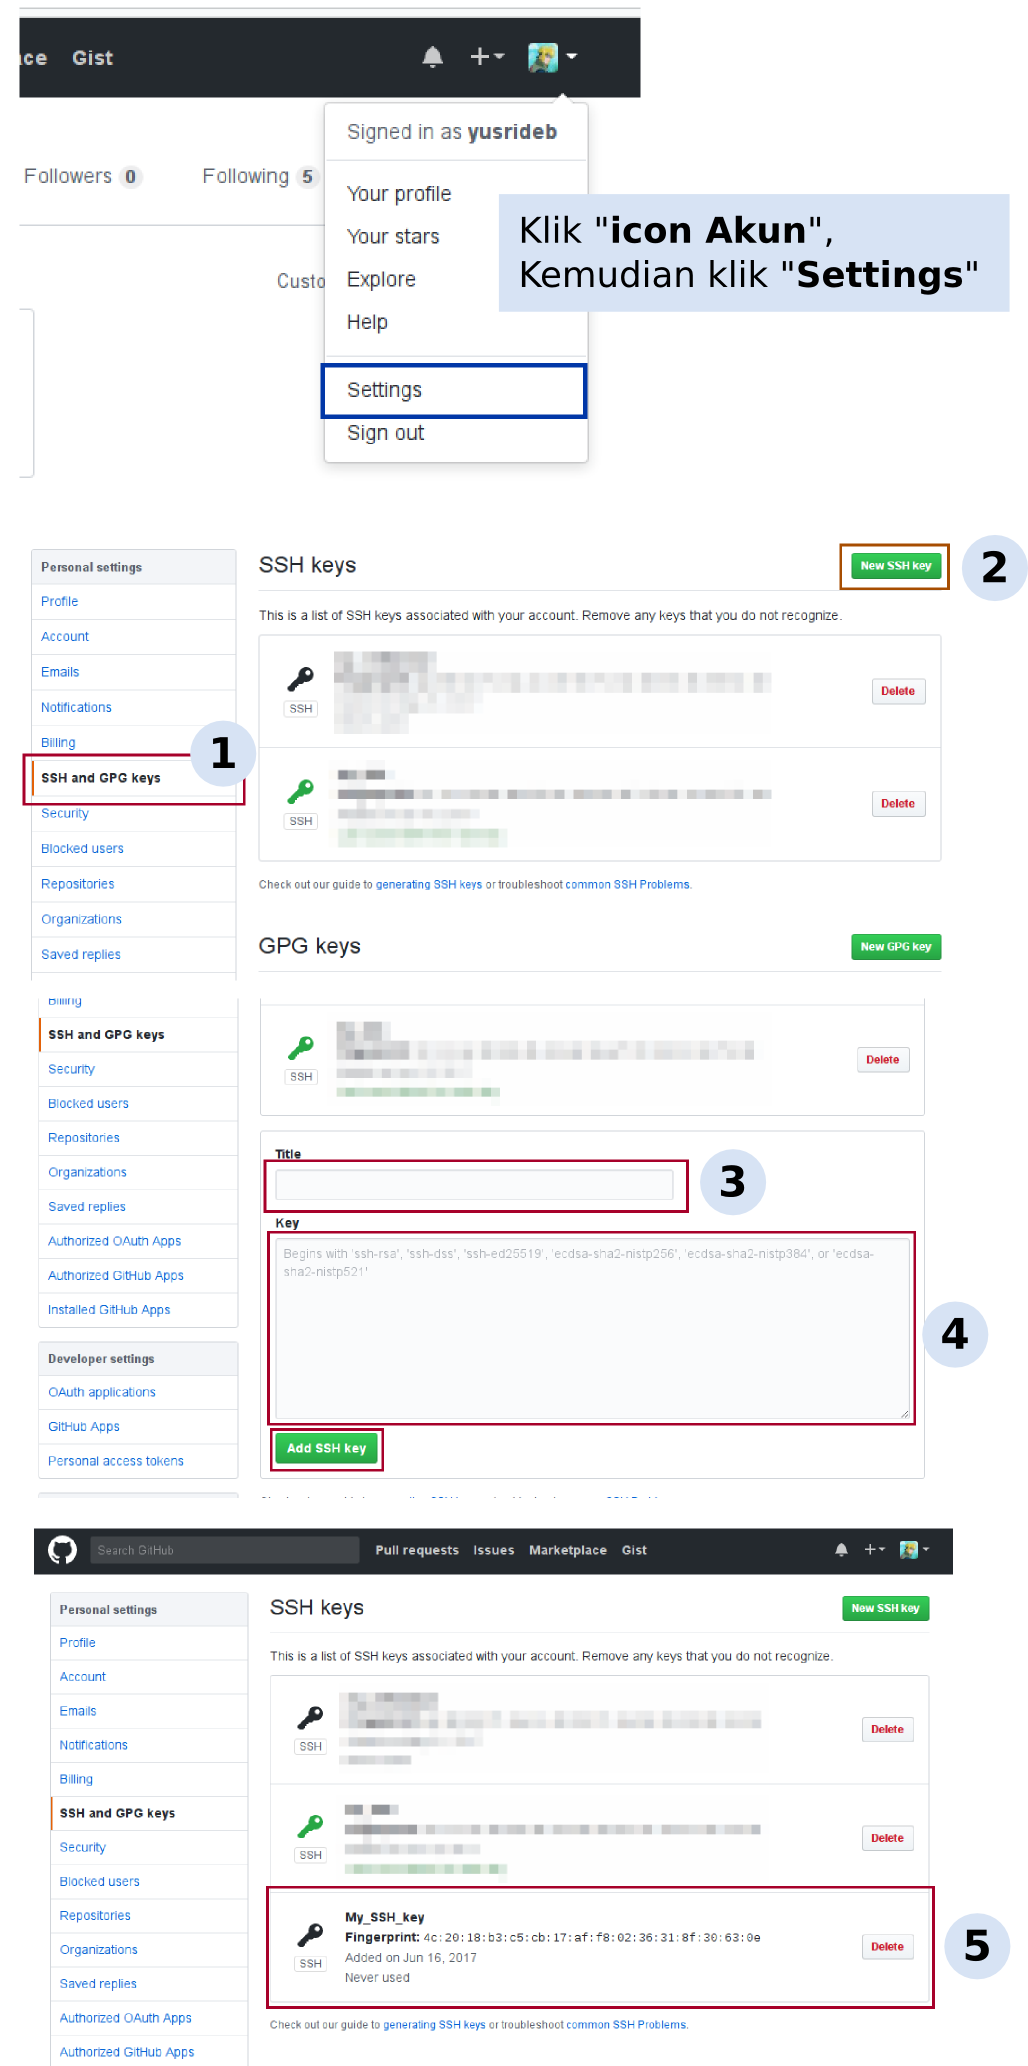
\includegraphics[width=7cm]{add-ssh-key-on-gtihub.png}
	\caption{Menambahkan \textit{Public SSH Key} di Akun Github}
	\label{fig:bab2_add-ssh-key-on-github}
\end{figure}

\begin{enumerate}
	\item Klik \textbf{SSH and GPG Keys}
	
	\item Klik \textbf{New SSH Key}
	
	\item Masukkan Nama \textit{SSH Key}, contohnya \textbf{My\_SSH\_key}
	
	\item Masukkan isi file \texttt{id\_rsa.pub} ke dalam form input \textbf{Key},
	Setelah itu klik \textbf{Add SSH Key}.
	
	\item Hasil akan tampil di Daftar \textbf{SSH Keys} seperti yang ditunjukkan oleh \textit{gambar \ref{fig:bab2_add-ssh-key-on-github}} di samping.
\end{enumerate}

\end{multicols}

\subsection{Metode Instalasi secara Manual}
\noindent
Instalasi manual untuk Module Perl \textbf{BlankOnDev} yang dimaksud disini yaitu instalasi dari Source Module CPAN yang dapat didownload pada halaman : \\ \footnotesize{\url{https://metacpan.org/release/BlankOnDev}} atau \\
\footnotesize{\url{https://github.com/yusrideb/BlankOnDev}}

\subsubsection{Install Dependensi Module}
\noindent
\normalsize
Jika versi \textbf{BlankOnDev Toos} yang terbaru sudah pernah di install sebelumnya, maka \textit{Dependensi} tidak pernah di install lagi.

\begin{lstlisting}[language=ShellBash]
sudo cpan -i Crypt::Blowfish Digest::MD5 
sudo cpan -i MIME::Base64 MIME::Base64::Perl JSON DateTime
sudo cpan -i GnuPG Hash::MultiValue Term::ReadKey LWP::UserAgent  
sudo cpan -i Text::SimpleTable::AutoWidth Capture::Tiny 
sudo cpan -i Capture::Tiny::Extended UNIVERSAL::ref parent
\end{lstlisting}

\subsubsection{Install Module Perl}
\noindent
Download Source dari halaman {\url{https://metacpan.org/release/BlankOnDev}, 
Contoh file source : "\textbf{BlankOnDev-0.1005.tar.gz}"

\begin{lstlisting}[language=ShellBash]
tar xzvf BlankOnDev-0.1005.tar.gz
cd BlankOnDev-0.1005
sudo perl Makefile.PL && make && make install && make clean.
\end{lstlisting}

\subsection{Metode Instalasi BlankOnDev dari CPAN Perl}
\noindent
Pada bagian ini \textit{Dependensi} beserta module utama akan di install secara otomatis. ketika perintah \texttt{cpan -i} di jalankan, seperti berikut :

\begin{lstlisting}[language=ShellBash]
sudo cpan -i BlankOnDev
\end{lstlisting}

\noindent
Proses instalasi ini akan berlangsung kurang lebih 10 menit dan bisa lebih tergantung kemampuan PC/Laptop Anda, karena selama proses instalasi berlangsung terdapat beberapa module-module dependensi yang melakukan kompilasi \textit{C Source}. 

\noindent
Dengan instalasi menggunakan perintah \texttt{cpan -i}, maka versi yang terinstall dari module dependensi atau module \textbf{BlankOnDev} yaitu versi terbaru, tidak seperti \textbf{Metode instalasi manual}, dimana versi module tergantung versi yang Anda download.

\noindent
Jika belum pernah menjalankan perintah \textbf{\texttt{cpan -i}} sebelumnya, maka pada saat perintah tersebut dijalankan pertama kali akan tampi \textbf{Form} seperti berikut :

\begin{figure}[H]
	\centering
	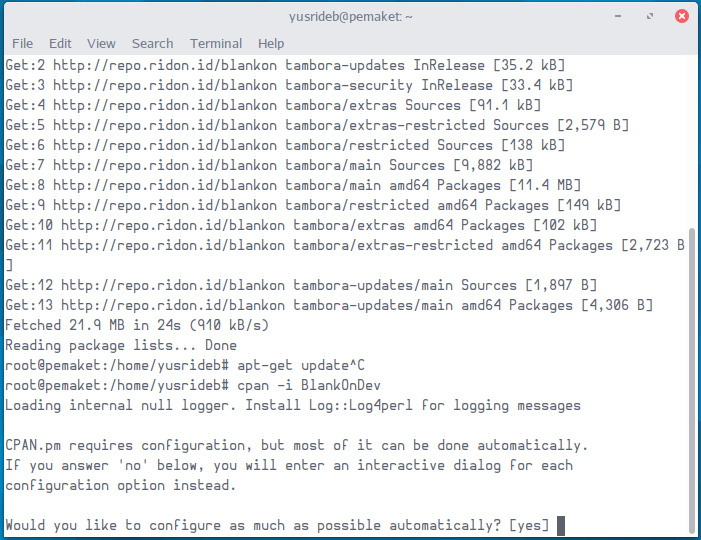
\includegraphics[width=10cm]{install-from-cpan-1.png}
	\caption{Form awal CPAN}
	\label{fig:bab2_form_awal_cpan}
\end{figure}

\noindent
Jika tampilkan form seperti gambar diatas, langsung saja tekan \textbf{Enter}.

\noindent
Jika sebelumnya anda sudah menggunakan perintah \textbf{\texttt{cpan -i}} maka instalasi module Perl akan dimulai, seperti berikut :

\begin{figure}[H]
	\centering
	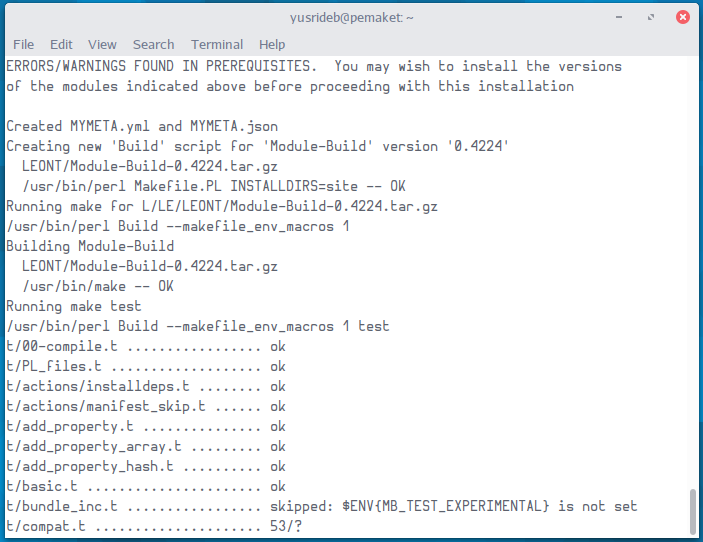
\includegraphics[width=10cm]{install-from-cpan-2.png}
	\caption{Instalasi Module Perl di mulai}
	\label{fig:bab2_start_install_module}
\end{figure}

\noindent
Jika dalam proses instalasi tidak ada yang bermasalah, maka akhir dari proses ini akan tampil seperti gambar berikut :

\begin{figure}[H]
	\centering
	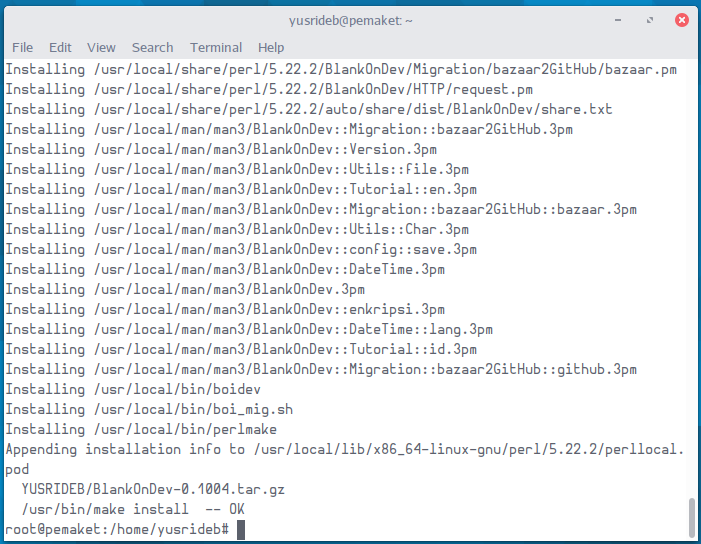
\includegraphics[width=12cm]{install-from-cpan-3_finish.png}
	\caption{Instalasi Module Selesai}
	\label{fig:bab1_finish_install_module}
\end{figure}

\section{Implementasi}
\label{subsec:implm}
\noindent
Pada bagian ini akan dijelaskan langkah-langkah penggunaan perintah \textbf{boidev}. Berikut gambaran penggunaan perintah \textbf{boidev} :

\subsection{Persiapan Migrasi Paket :}
\begin{enumerate}
	\item \textbf{Step 1} - Perintah yang dijalankan sebelum menjalankan perintah \textbf{boidev} lainnya yaitu perintah \textbf{\texttt{boidev config}} untuk konfigurasi program seperti :
	\label{itm:pre_step1}
	\begin{itemize}
		\item Memasukkan nama \textbf{time zone},
		\item Memasukkan alamat \textbf{Email} yang digunakan di akun \textit{Github} dan maupun alamat \textbf{Email} untuk generate key dengan GnuPG, dan
		\item Generate Key GnuPG.
	\end{itemize}
	
	\item \textbf{Step 2} - Menggunakan perintah \texttt{boidev mig\_prepare}. Perintah ini akan melakukan persiapan sebelum Migrasi paket, yaitu :
	\label{itm:pre_step2}
	\begin{itemize}
		\item Config github, seperti \textit{nama}, \textit{Alamat Email}, dan \textit{Cache Username dan Password}
		
		\item Opsi Generate Key GnuPG.\\
		
		\item Memasukkan alamat bazaar repositori\\ (example: \textbf{http://dev.blankonlinux.or.id/browser/tambora})

		\item Memasukkan alamat github repositori\\ (example: \textbf{https://github.com/blankon-packages})	
	\end{itemize}
	
	\item \textbf{Step 3} -  Menambahkan \textit{Group Paket} untuk \textit{Paket-paket} yang akan di migrasi ke repositori github. Perintah yang digunakan antara lain :
	\label{itm:pre_step3}
	\begin{enumerate}
		\item perintah \texttt{boidev bzr2git addpkg-group},
		\item perintah \texttt{boidev bzr2git addpkg} dan
		\item perintah \texttt{boidev bzr2git addpkg-file}
	\end{enumerate}
\end{enumerate}

\subsection{Proses Migrasi Paket :}
\begin{enumerate}
	
	\item \textbf{Skema split} - Branch, convert format, dan push dilakukan terpisah, dengan perintah :
	\label{itm:metode_split}
	\begin{enumerate}
		\item perintah \texttt{boidev bzr2git branch}
		\item perintah \texttt{boidev bzr2git bzr-cgit}
		\item perintah \texttt{boidev bzr2git git-push}
		\item perintah \texttt{boidev bzr2git git-check}
	\end{enumerate}
	
	\item \textbf{Skema one-time} - Branch, convert format, dan push dilakukan sekaligus dengan satu perintah yaitu dengan perintah \texttt{boidev bzr2git}.
	\label{itm:metode_one-time}
\end{enumerate}

\section{Persiapan Migrasi Paket}
\subsection{Persiapan Migrasi Paket - \texttt{boidev config}}
\label{implm_1}
\noindent
Jalankan perintah \texttt{boidev config} pada \textbf{User biasa} bukan \textit{User root} seperti berikut :

\begin{lstlisting}[language=ShellBash]
$ boidev config
\end{lstlisting}

\noindent
Kemudian proses \texttt{apt-get update} akan berjalan seperti berikut :

\begin{lstlisting}[language=ShellBash]
Hit:1 http://repo.ridon.id/blankon tambora InRelease
Hit:2 http://repo.ridon.id/blankon tambora-updates InRelease
Hit:3 http://repo.ridon.id/blankon tambora-security InRelease
Reading package lists... Done                      
Reading package lists... Done

\end{lstlisting}

\noindent
Setelah proses diatas maka akan di install beberapa paket-paket yang dibutuhkan oleh \textbf{Tim Pemaket} selesai terinstalasi. Kemudian akan tampil Form seperti berikut dan masukkan nomor sesuai dengan yang ada di \textbf{List}.

\begin{lstlisting}[language=ShellBash]

List TimeZone : 
1. WIB 
2. WITA 
3. WIT 
Enter your time zone [WITA] : 2

\end{lstlisting}

\noindent
Form berikut ini isi sesuai petunjuk yang diberi tanda \textbf{\#}.

\begin{lstlisting}[language=ShellBash]

# Nama Lengkap
Enter your name : Achmad Yusri Afandi

# Email Github
Enter your email address Github Account : linuxer08@gmail.com

# Email yang digunakan saat generate GnuPG
Enter your email address for GnuPG Generate Key : yusrideb@cpan.org


# Masukkan Passphrase seperti saat menjalankan gpg --gen-key
Enter Passphrase gpg : 

\end{lstlisting}

\subsection{Dengan perintah \texttt{boidev mig\_prepare}}
\label{implm_2}
\noindent
Jalankan perintah berikut :

\begin{lstlisting}[language=ShellBash]
$ boidev mig_prepare
\end{lstlisting}

\noindent Setelah itu akan tampil form seperti pada \texttt{boidev config} :

\begin{lstlisting}[language=ShellBash]

List TimeZone : 
1. WIB
2. WITA
3. WIT
Enter your time zone [WITA] : 2

\end{lstlisting}

\noindent
Form berikut yaitu form \textbf{Github config} :

\begin{lstlisting}[language=ShellBash]
You want reconfig github [y/n]:
\end{lstlisting}

\subsubsection{Penjelasan form \textbf{reconfig github} :}

\begin{itemize}
	\item Jika inputnya \textbf{\texttt{y}} maka akan tampil form config github seperti berikut :
	
	\begin{lstlisting}[language=ShellBash]
	# Masukkan nama jika, ingin mengubah nama yang sudah
	# tersimpan pada system. Jika tidak langsung tekan Enter
	Enter your github fullname [Achmad Yusri Afandi] : 
	
	# Masukkan email github, jika ingin mengubah nama yang sudah
	# tersimpan pada system. Jika tidak langsung tekan Enter
	Enter your github email [linuxer08@gmail.com] : 
	\end{lstlisting}
	
	\item Jika inputnya \textbf{\texttt{n}} maka akan dilanjutkan ke form berikutnya.
\end{itemize}

\subsubsection{Form GnuPG Generate Key :}

\begin{lstlisting}[language=ShellBash]
You want GnuPG Generate key [y/n]: 
\end{lstlisting}

\begin{itemize}
	\item Jika jawaban \textbf{\texttt{y}} :
	\begin{lstlisting}[language=ShellBash]
	# Masukkan nama jika, ingin mengubah nama yang sudah
	# tersimpan pada system. Jika tidak langsung tekan Enter
	Enter Name [Achmad Yusri Afandi] : 
	
	# Masukkan email untuk GnuPG, jika ingin mengubah nama yang
	# sudah tersimpan pada system. 
	# Jika tidak langsung tekan Enter
	Enter E-mail [yusrideb@cpan.org] : 
	\end{lstlisting}
	
	Setelah form diatas, maka akan tampil form untuk mengubah \textit{passphrase GnuPG} atau tidak, Jika jawabannya "\texttt{\textbf{y}}" maka akan tampil form untuk memasukkan passphrase, jika tidak, maka proses \textbf{Generate Key GnuPG} akan dilanjutkan.
	
	\begin{lstlisting}[language=ShellBash]
	You want to enter different passphrase GnuPG ? [y or n] n
	\end{lstlisting}
	
	\noindent
	Setelah form diatas, maka akan tampil hasil \textbf{Generate Key GnuPG} :
	
	\begin{lstlisting}[language=ShellBash2]
	Enter passphrase : pub   1024R/243741DF 2017-06-12
	Key fingerprint = 8891 3EF3 6E21 C298 B7B6  0F0A 1380 3397 2437 41DF
	uid                  Achmad Yusri Afandi <yusrideb@cpan.org>
	sub   1024R/EF69A466 2017-06-12
	\end{lstlisting}
	
	\item Jika jawaban \textbf{\texttt{n}}, maka akan langsung ke form untuk memasukkan URL.
	
\end{itemize}

\pagebreak
\subsubsection{Form URL Repositori Bazaar dan Github :}

\begin{itemize}
	\item Jika data \textbf{belum ada} :
	
	\begin{lstlisting}[language=ShellBash2]
	
	# Masukkan URL repositori bazaar, contohnya :
	# http://dev.blankonlinux.or.id/browser/tambora
	#
	Enter bzr url : 
	
	# Masukkan URL repositori Github, contohnya :
	# git@github.com:blankon-packages
	#
	Enter git url : 
	
	\end{lstlisting}
	
	\item Jika data \textbf{sudah ada} :
	
	\begin{lstlisting}[language=ShellBash2]
	
	# Masukkan URL  URL repositori bazaar jika anda ingin 
	# mengubah alamatnya. Jika tidak, langsung saja tekan Enter.
	#
	Enter bzr url [http://dev.blankonlinux.or.id/browser/tambora] : 
	
	# Masukkan URL  URL repositori github jika anda ingin 
	# mengubah alamatnya. Jika tidak, langsung saja tekan Enter.
	#
	Enter git url [git@github.com:blankon-packages] : 
	
	\end{lstlisting}
	
\end{itemize}

\subsection{Menambahkan Group paket dan nama paket}
\label{implm_3}
\noindent
Seperti yang telah dijelaskan pada upabab \textit{\ref{subsec:implm}. Implementasi - \textit{Persiapan Migrasi Paket}, di halaman \pageref{itm:pre_step3}} yaitu menggunakan perintah "\texttt{boidev bzr2git addpkg-group}", "\texttt{boidev bzr2git addpkg}" dan "\texttt{boidev bzr2git addpkg-file}".

\subsubsection{Menambahkan Group Paket}
\label{subsubsec:addpkg-group}
\noindent
Untuk menambahkan group paket gunakan perintah berikut :

\begin{lstlisting}[language=ShellBash]
$ boidev bzr2git addpkg-group 
\end{lstlisting}

\noindent
kemudian akan tampil form seperti berikut :

\begin{lstlisting}[language=ShellBash]
Enter new group name : github-6
\end{lstlisting}

\noindent
Atau langsung masukkan nama paket group, contoh nama group paket \textbf{githb-6}

\begin{lstlisting}[language=ShellBash]
$ boidev bzr2git addpkg-group github-6
\end{lstlisting}

\noindent
Outputnya seperti berikut:

\begin{lstlisting}[language=ShellBash]

Success added package group with name "github-6"
\end{lstlisting}

\subsubsection{Melihat daftar Group paket}
\label{subsubsec:list-pkg-group}
\noindent
Jalankan perintah berikut :

\begin{lstlisting}[language=ShellBash]
$ boidev bzr2git list-pkg-group
\end{lstlisting}

\noindent
dan outputnya seperti berikut :

\begin{lstlisting}[language=ShellBash]

Exists Groups : 
------------------------------------------------------
- github-6

______________________________________________________
\end{lstlisting}

\subsubsection{Menambahkan nama paket}
\label{subsubsec:addpkg}
\noindent
Jalankan perintah berikut :

\begin{lstlisting}[language=ShellBash]
$ boidev bzr2git addpkg
\end{lstlisting}

\noindent
kemudian akan tampil form seperti berikut :

\begin{lstlisting}[language=ShellBash]
# Masukkan nomor list group
#
Choose Group Packages.
1. github-6
Enter Number choice : 1

# Masukkan nama group 
#
Enter New Packages : gnome-font-viewer
\end{lstlisting}

\noindent
atau langsung masukkan nama paket :

\begin{lstlisting}[language=ShellBash]
$ boidev bzr2git addpkg gnome-font-viewer
\end{lstlisting}

\noindent
Form pilih nama group :

\begin{lstlisting}[language=ShellBash]
# Masukkan nomor list group
#
Choose Group Packages.
1. github-6
Enter Number choice : 1
\end{lstlisting}

\subsubsection{Menambahkan nama paket dari file}
\label{subsubsec:addpkg-file}
\noindent
Cara ini digunakan jika terdapat lebih dari 1 nama paket yang akan ditambahkan contohnya :

\begin{lstlisting}[language=ShellBash]
gnome-documents
gnome-font-viewer
gnome-icon-theme
gnome-icon-theme-symbolic
gnome-keyring
gnome-logs
gnome-menus
gnome-music
gnome-online-accounts
gnome-packagekit
gnome-photos
gnome-pkg-tools
gnome-power-manager
gnome-screensaver
gnome-screenshot
gnome-shell
gnome-settings-daemon
gnome-shell-extensions
gnome-software
\end{lstlisting}

\noindent
Daftar nama paket tersebut dimasukkan kedalam file yang berekstensi \textbf{.boikg}, karena program hanya akan membaca file yang berekstensi \textbf{.boikg}

\noindent
Setelah daftar \textit{nama paket} dimasukkan dalam file, kemudian jalankan perintah berikut dengan syntax :\\ {\small \texttt{boidev bzr2git addpkg-file <lokasi\_file\/nama\_file.bokg>}}\\
Contoh lokasi file di : {\small \texttt{/home/yusrideb/github-6.boikg}}

\begin{lstlisting}[language=ShellBash]
$ boidev bzr2git addpkg-file /home/yusrideb/github-6.boikg
\end{lstlisting}

\noindent
Kemudian akan tampil form untuk memilih group paket :

\begin{lstlisting}[language=ShellBash]
# Masukkan nomor list :
#
Choose Group Packages.
1. github-6
Enter Number choice : 1
\end{lstlisting}

\noindent
Output :

\begin{lstlisting}[language=ShellBash]

"gnome-documents" has success added.
"gnome-font-viewer" has success added.
"gnome-icon-theme" has success added.
"gnome-icon-theme-symbolic" has success added.
"gnome-keyring" has success added.
"gnome-logs" has success added.
"gnome-menus" has success added.
"gnome-music" has success added.
"gnome-online-accounts" has success added.
"gnome-packagekit" has success added.
"gnome-photos" has success added.
"gnome-pkg-tools" has success added.
"gnome-power-manager" has success added.
"gnome-screensaver" has success added.
"gnome-screenshot" has success added.
"gnome-shell" has success added.
"gnome-settings-daemon" has success added.
"gnome-shell-extensions" has success added.
"gnome-software" has success added.

19 packages has added...

\end{lstlisting}

\subsubsection{Melihat Daftar Paket}
\noindent
Untuk melihat list paket, menggunakan perintah : 
\begin{enumerate}
	\item {\small \texttt{boidev bzr2git list-pkg}}
	\item {\small \texttt{boidev bzr2git list-pkg <nama\_group\_paket>}}
\end{enumerate}

\noindent
\textbf{Perintah {\small \texttt{boidev bzr2git list-pkg}}}

\begin{lstlisting}[language=ShellBash]
$ boidev bzr2git list-pkg
\end{lstlisting}

\noindent
Kemudian akan form untuk memilih group paket, setelah itu akan tampil daftar paket seperti berikut:

\begin{figure}[H]
	\centering
	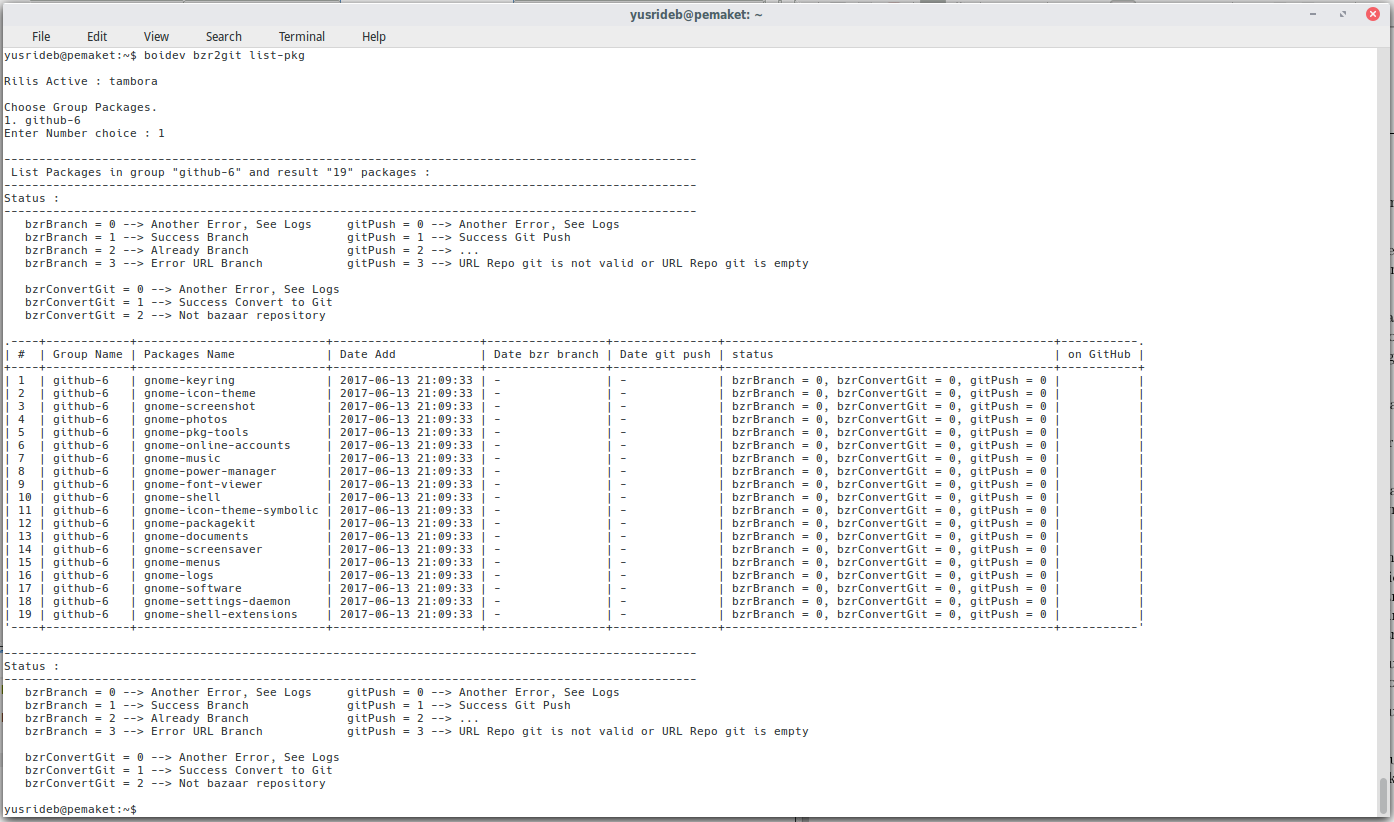
\includegraphics[width=12cm]{boidev_bzr2git_list-pkg.png}
	\caption{Daftar Paket yang telah ditambahkan dengan nama group \textbf{github-6}}
	\label{fig:bab2_list-pkg}
\end{figure}

\noindent
\textbf{Perintah {\small \texttt{boidev bzr2git list-pkg <nama\_group\_paket>}}}

\begin{lstlisting}[language=ShellBash]
$ boidev bzr2git list-pkg github-6
\end{lstlisting}

\noindent
Output :
\begin{figure}[H]
	\centering
	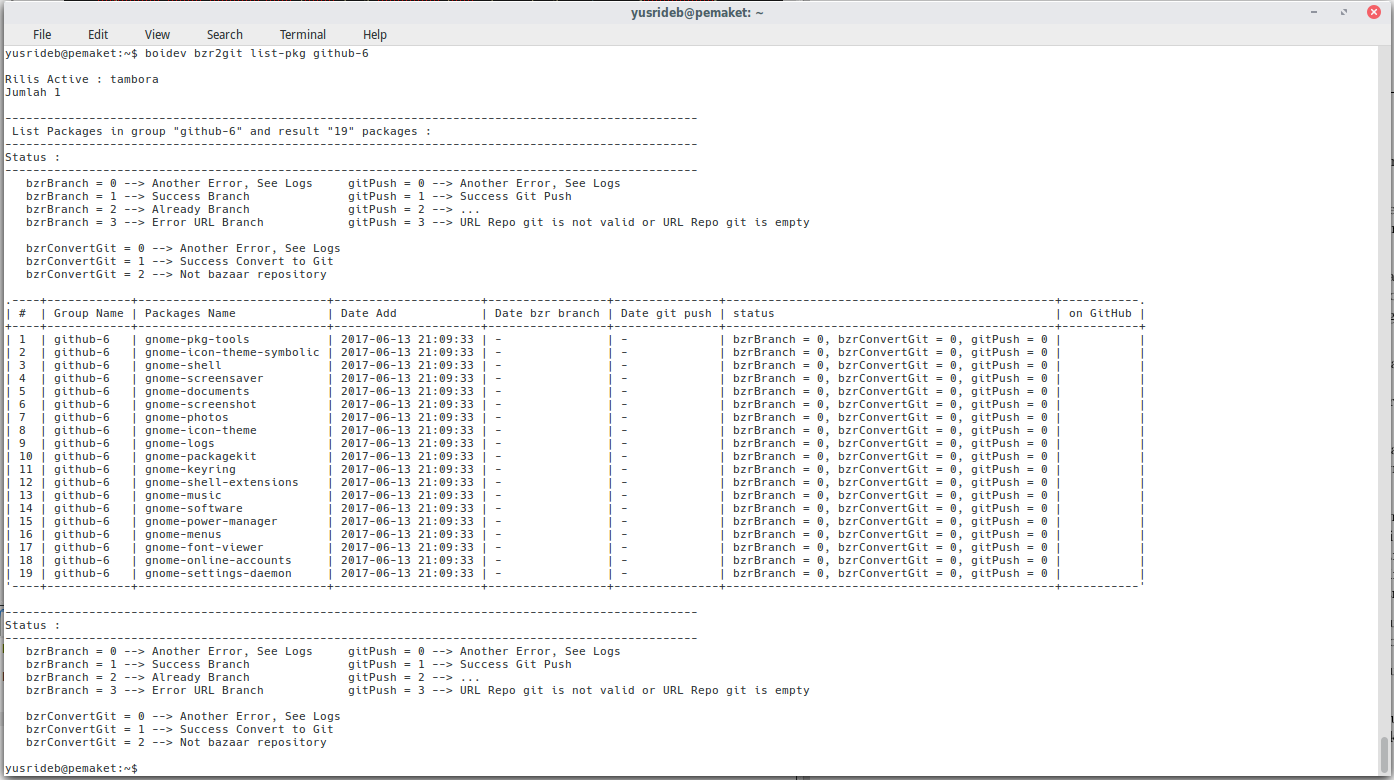
\includegraphics[width=12cm]{boidev_bzr2git_list-pkg_groupName.png}
	\caption{Daftar Paket yang telah ditambahkan dengan nama group \textbf{github-6}}
	\label{fig:bab2_list-pkg_bygrp}
\end{figure}

\section{Proses Migrasi Paket}
\label{sec:pre_impl_pros_mig}
\noindent
Proses yang dilakukan disini yaitu penggunaan perintah-perintah seperti contoh berikut. Perintah \textbf{boidev} bertujuan untuk meminimalisir kesalahan penulisan perintah ataupun kesalahan penulisan \textit{nama paket}.

\begin{lstlisting}[language=ShellBash2, caption=Perintah Migrasi, label=lst:migrasi_manual]

bzr branch http://dev.blankonlinux.or.id/browser/tambora/<nama_paket>
cd <nama_paket>
git init
bzr fast-export $(pwd) | git fast-import
git reset HEAD
rm -rf .bzr
git remote add origin git@github.com:blankon-packages/<nama_paket>.git
git push -u origin master
git checkout -b tambora
git push -u origin tambora
git branch -a
\end{lstlisting}

\subsection{Migrasi Paket dengan \textbf{Metode Split}}
\label{implm_4}
\noindent
Seperti yang telah dijelaskan pada upabab \textit{\ref{subsec:implm}. Implementasi, di halaman \pageref{itm:metode_split}}, Bahwa \textit{metode} ini melakukukan \textit{branch paket}, \textit{convert format ke git}, dan \textit{push ke git} secara terpisah. Seperti metode migrasi yang dilakukan secara manual seperti yang ditunjukkan pada \textit{listing - \ref{lst:migrasi_manual} Perintah Migrasi} diatas. Berikut langkah-langkahnya :

\subsubsection{Perintah {\small \texttt{boidev bzr2git branch}}}
\noindent
Perintah yang dapat digunakan yaitu :
\begin{itemize}
	\item {\small \texttt{boidev bzr2git branch}}
	\item {\small \texttt{boidev bzr2git branch <nama\_group\_paket>}}
\end{itemize}

\noindent
Proses yang akan tampil ketika salah satu perintah diatas dijalankan yaitu :

\begin{lstlisting}[language=ShellBash2]
# Masuk sesuai dengan nomor list
#
Choose Group Packages.
1. github-6
Enter Number choice : 1

# Jika jawabannya "y" maka jika nama paket sudah ada akan dihapus.
# Jika jawabannya "n" maka `branch` tidak akan dilakukan pada 
# nama paket yang sudah ada.
#
You want to re-branch if packages is exists on local directory [y/n] : y

Branch : "gnome-screensaver"
Result Action branch : 1

Branch : "gnome-icon-theme"
Result Action branch : 1

Branch : "gnome-menus"
Result Action branch : 1

Branch : "gnome-keyring"
Result Action branch : 1

Branch : "gnome-settings-daemon"
Result Action branch : 1

Branch : "gnome-online-accounts"
Result Action branch : 1

Branch : "gnome-shell-extensions"
Result Action branch : 1

Branch : "gnome-screenshot"
Result Action branch : 1

Branch : "gnome-font-viewer"
Result Action branch : 1

Branch : "gnome-logs"
Result Action branch : 1

Branch : "gnome-shell"
Result Action branch : 1

Branch : "gnome-music"
Result Action branch : 1

Branch : "gnome-icon-theme-symbolic"
Result Action branch : 1

Branch : "gnome-power-manager"
Result Action branch : 1

Branch : "gnome-documents"
Result Action branch : 1

Branch : "gnome-pkg-tools"
Result Action branch : 1

Branch : "gnome-software"
Result Action branch : 1

Branch : "gnome-photos"
Result Action branch : 1

Branch : "gnome-packagekit"
Result Action branch : 1

==================== bzr branch has finished ====================

\end{lstlisting}

\subsubsection{Perintah {\small \texttt{boidev bzr2git bzr-cgit}}}
\noindent
Perintah yang dapat digunakan yaitu :
\begin{itemize}
	\item {\small \texttt{boidev bzr2git bzr-cgit}}
	\item {\small \texttt{boidev bzr2git bzr-cgit <nama\_group\_paket>}}
\end{itemize}

\noindent
Proses yang akan tampil ketika salah satu perintah diatas dijalankan yaitu :

\begin{lstlisting}[language=ShellBash2]
# Masuk sesuai dengan nomor list
#
Choose Group Packages.
1. github-6
Enter Number choice : 1

Converting .... 

Action Convert gnome-logs : 1
Action Convert gnome-online-accounts : 1
Action Convert gnome-keyring : 1
Action Convert gnome-settings-daemon : 1
Action Convert gnome-screensaver : 1
Action Convert gnome-packagekit : 1
Action Convert gnome-power-manager : 1
Action Convert gnome-screenshot : 1
Action Convert gnome-font-viewer : 1
Action Convert gnome-music : 1
Action Convert gnome-icon-theme : 1
Action Convert gnome-software : 1
Action Convert gnome-shell : 1
Action Convert gnome-menus : 1
Action Convert gnome-pkg-tools : 1
Action Convert gnome-icon-theme-symbolic : 1
Action Convert gnome-documents : 1
Action Convert gnome-photos : 1
Action Convert gnome-shell-extensions : 1

======= Packages in group "github-6" has been finished to convert ========
\end{lstlisting}

\subsubsection{Perintah {\small \texttt{boidev bzr2git git-push}}}
\noindent
Perintah yang dapat digunakan yaitu :
\begin{itemize}
	\item {\small \texttt{boidev bzr2git git-push}}
	\item {\small \texttt{boidev bzr2git git-push <nama\_group\_paket>}}
\end{itemize}

\noindent
Proses yang akan tampil ketika salah satu perintah diatas dijalankan yaitu :

\begin{lstlisting}[language=ShellBash2]
# Masuk sesuai dengan nomor list
#
Choose Group Packages.
1. github-6
Enter Number choice : 1

Push to github .... 

# Jika tampil form seperti berikut
# masukkan passphrase yang digunakan saat membuat
# Public SSH Key :
Enter passphrase for key '/home/yusrideb/.ssh/id_rsa': 

gitpush : gnome-music
Action Git push for packages gnome-music : 1 
gitpush : gnome-software
Action Git push for packages gnome-software : 1 
gitpush : gnome-packagekit
Action Git push for packages gnome-packagekit : 1 
gitpush : gnome-icon-theme-symbolic
Action Git push for packages gnome-icon-theme-symbolic : 1 
gitpush : gnome-documents
Action Git push for packages gnome-documents : 1 
gitpush : gnome-power-manager
Action Git push for packages gnome-power-manager : 1 
gitpush : gnome-online-accounts
Action Git push for packages gnome-online-accounts : 1 
gitpush : gnome-settings-daemon
Action Git push for packages gnome-settings-daemon : 1 
gitpush : gnome-keyring
Action Git push for packages gnome-keyring : 1 
gitpush : gnome-font-viewer
Action Git push for packages gnome-font-viewer : 1 
gitpush : gnome-menus
Action Git push for packages gnome-menus : 1 
gitpush : gnome-screensaver
Action Git push for packages gnome-screensaver : 1 
gitpush : gnome-icon-theme
Action Git push for packages gnome-icon-theme : 1 
gitpush : gnome-shell
Action Git push for packages gnome-shell : 1 
gitpush : gnome-photos
Action Git push for packages gnome-photos : 1 
gitpush : gnome-screenshot
Action Git push for packages gnome-screenshot : 1 
gitpush : gnome-pkg-tools
Action Git push for packages gnome-pkg-tools : 1 
gitpush : gnome-shell-extensions
Action Git push for packages gnome-shell-extensions : 1 
gitpush : gnome-logs
Action Git push for packages gnome-logs : 1 

======= Packages in group "github-6" has been finished to git push =======
\end{lstlisting}

\subsubsection{Perintah {\small \texttt{boidev bzr2git git-check}}}
\noindent
Perintah yang dapat digunakan yaitu :
\begin{itemize}
	\item {\small \texttt{boidev bzr2git git-check}}
	\item {\small \texttt{boidev bzr2git git-check <nama\_group\_paket>}}
\end{itemize}

\noindent
Proses yang akan tampil ketika salah satu perintah diatas dijalankan yaitu :

\begin{lstlisting}[language=ShellBash2]
# Masuk sesuai dengan nomor list
#
Choose packages group : 
------------------------------------------------------
1. github-6                  [20]
------------------------------------------------------
Enter number of group name : 1

Check repo on github for all packages : 
Check Repo [gnome-music] on github : repo_github = master, tambora 
Check Repo [gnome-icon-theme-symbolic] on github : repo_github = master, tambora 
Check Repo [gnome-settings-daemon] on github : repo_github = master, tambora 
Check Repo [gnome-menus] on github : repo_github = master, tambora 
Check Repo [gnome-online-accounts] on github : repo_github = master, tambora 
Check Repo [gnome-shell-extensions] on github : repo_github = master, tambora 
Check Repo [gnome-documents] on github : repo_github = master, tambora 
Check Repo [gnome-keyring] on github : repo_github = master, tambora 
Check Repo [gnome-icon-theme] on github : repo_github = master, tambora 
Check Repo [gnome-power-manager] on github : repo_github = master, tambora 
Check Repo [gnome-logs] on github : repo_github = master, tambora 
Check Repo [gnome-photos] on github : repo_github = master, tambora 
Check Repo [gnome-shell] on github : repo_github = master, tambora 
Check Repo [gnome-font-viewer] on github : repo_github = master, tambora 
Check Repo [gnome-pkg-tools] on github : repo_github = master, tambora 
Check Repo [gnome-software] on github : repo_github = master, tambora 
Check Repo [gnome-screenshot] on github : repo_github = master, tambora 
Check Repo [gnome-screensaver] on github : repo_github = master, tambora 
Check Repo [gnome-packagekit] on github : repo_github = master, tambora 

======= Git Check All Packages on Group [github-6] has finished =======
\end{lstlisting}

\subsubsection{Melihat hasil Migrasi}
\noindent
Jika anda ingin melihat hasil migrasi gunakan perintah\\ {\small \texttt{boidev bzr2git list-pkg <nama\_group\_paket>}} seperti berikut :

\begin{lstlisting}[language=ShellBash]
$ boidev mig_prepare
\end{lstlisting}

\noindent
Output :

\begin{figure}[H]
	\centering
	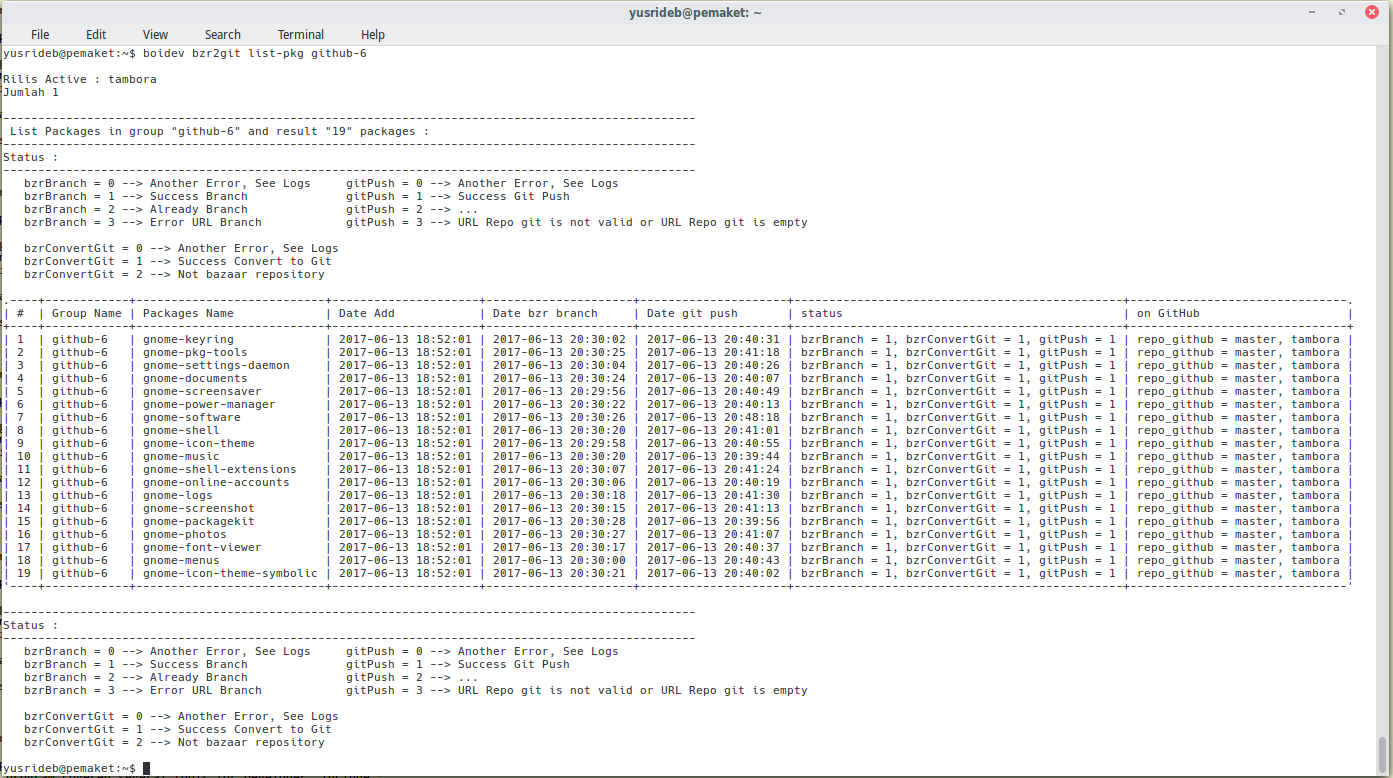
\includegraphics[width=13cm]{boidev_bzr2git_list-pkg-check.png}
	\caption{List Packages}
	\label{fig:bab2_list_pkg_check}
\end{figure}

\begin{figure}[H]
	\centering
	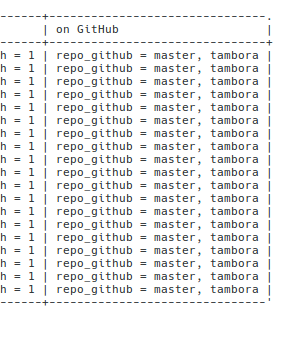
\includegraphics[width=5cm]{boidev_bzr2git_list-pkg-check_zoom.png}
	\caption{List Packages bagian hasil git-check}
	\label{fig:bab2_list_pkg_check_zoom}
\end{figure}

\subsection{Migrasi Paket dengan \textbf{Skema One-time}}
\label{implm_5}
\noindent 
Seperti yang telah dijelaskan pada upabab \textit{\ref{subsec:implm}. Implementasi, di halaman \pageref{itm:metode_one-time}}, Bahwa \textit{metode} ini melakukukan \textit{branch paket}, \textit{convert format ke git}, dan \textit{push ke git} sekaligus dengan perintah {\small \textit{\texttt{boidev bzr2git}}}. Skema ini menjalankan seluruh perintah yang terdapat pada \textit{listing - \ref{lst:migrasi_manual} Perintah Migrasi}, Berikut langkah-langkahnya:

\subsubsection{Migrasi 1 paket}

\begin{lstlisting}[language=ShellBash2]

# Untuk Migrasi 1 paket, maka masukkan nomor "3"
#
---------------------------------------------------------------------------
Choose Action : 
---------------------------------------------------------------------------
1. All Packages
2. Specific Group Packages
3. Single Packages
Answer: 3

# Contoh paket yaitu "gnome-keyring"
# 
Enter packages name : gnome-keyring

Branch : "gnome-keyring"
[success] Action "bzr branch -> gnome-keyring" : 1
[success] Action "bzr convert git -> gnome-keyring" 1 


# Jika tampil form seperti berikut
# masukkan passphrase yang digunakan saat membuat
# Public SSH Key :
Enter passphrase for key '/home/yusrideb/.ssh/id_rsa': 

[success] Action "git push -> gnome-keyring" 1
[success] Action "git check -> gnome-keyring" repo_github = master, tambora

====== Migration packages "gnome-keyring" has been finished ======
\end{lstlisting}

\subsubsection{Migrasi Berdasarkan group paket}

\begin{lstlisting}[language=ShellBash2]

# Untuk Migrasi paket berdasarkan group, maka masukkan nomor "2"
#
---------------------------------------------------------------------------
Choose Action : 
---------------------------------------------------------------------------
1. All Packages
2. Specific Group Packages
3. Single Packages
Answer: 2

# Masukkan sesuai nomor list
# Pada contoh ini yaitu nomor "3"
#
Choose packages group : 
------------------------------------------------------
1. github-end-2              [10]
2. github-6                  [19]
3. github-end-3              [5]
4. github-end-1              [10]
------------------------------------------------------
Enter number of group name : 3

Doing migration ...

Branch : "ntfs-3g"
[success] Action "bzr branch -> ntfs-3g" : 1
[success] Action "bzr convert git -> ntfs-3g" 1
[success] Action "git push -> ntfs-3g" 1
[success] Action "git check -> ntfs-3g" repo_github = master, tambora
------------------------------------------------------------------------

Branch : "opencv"
[success] Action "bzr branch -> opencv" : 1
[success] Action "bzr convert git -> opencv" 1
[success] Action "git push -> opencv" 1
[success] Action "git check -> opencv" repo_github = master, tambora
------------------------------------------------------------------------
Branch : "nss"
[success] Action "bzr branch -> nss" : 1
[success] Action "bzr convert git -> nss" 1
[success] Action "git push -> nss" 1
[success] Action "git check -> nss" repo_github = master, tambora
------------------------------------------------------------------------
Branch : "nvidia-firmware"
[success] Action "bzr branch -> nvidia-firmware" : 1
[success] Action "bzr convert git -> nvidia-firmware" 1
[success] Action "git push -> nvidia-firmware" 1
[success] Action "git check -> nvidia-firmware" repo_github = master, tambora
------------------------------------------------------------------------
Branch : "notify-osd"
[success] Action "bzr branch -> notify-osd" : 1
[success] Action "bzr convert git -> notify-osd" 1
[success] Action "git push -> notify-osd" 1
[success] Action "git check -> notify-osd" repo_github = master, tambora
------------------------------------------------------------------------

======== Migration all packages in group "github-end-3" has been finished ========

\end{lstlisting}

\subsubsection{Migrasi Semua paket dalam list}

\begin{lstlisting}[language=ShellBash2]

# Untuk Migrasi semua paket, maka masukkan nomor "1"
#
---------------------------------------------------------------------------
Choose Action : 
---------------------------------------------------------------------------
1. All Packages
2. Specific Group Packages
3. Single Packages
Answer: 3

# Jika jawaban "y" maka semua paket yang terdaftar akan dimigrasi secara otomatis
# Jika jawaban "n" maka akan muncul pertanyaan sebelum paket dalam group di migrasi
# 
You want migration all packages with automatically ? [y or n] n

List Group packages to Migration : 
---------------------------------------------
1. github-end-1         [10]
2. github-end-2         [10]
3. github-6             [19]
4. github-end-3         [5]
---------------------------------------------

You want to migration all packages in group "github-end-1 [10]" ? [y or n] y

[migration] All packages in group "github-end-1" 
------------------------------------------------------------------------
Action re-branch for packages "live-boot" 
[success] Action "bzr branch -> live-boot" : 1
[success] Action "bzr convert git -> live-boot" 1
[success] Action "git push -> live-boot" 1
[success] Action "git check -> live-boot" repo_github = master, tambora
------------------------------------------------------------------------
Branch : "manokwari"
[success] Action "bzr branch -> manokwari" : 1
[success] Action "bzr convert git -> manokwari" 1
[success] re-Action "bzr convert git -> manokwari" 1
[success] Action "re-git push -> manokwari" 
[success] Action "git check -> manokwari" repo_github = master, tambora
------------------------------------------------------------------------
Branch : "linux-ntfs"
[success] Action "bzr branch -> linux-ntfs" : 1
[success] Action "bzr convert git -> linux-ntfs" 1
[success] Action "git push -> linux-ntfs" 1
[success] Action "git check -> linux-ntfs" repo_github = master, tambora
------------------------------------------------------------------------
Branch : "lvm2"
[success] Action "bzr branch -> lvm2" : 1
[success] Action "bzr convert git -> lvm2" 1
[success] Action "git push -> lvm2" 1
[success] Action "git check -> lvm2" repo_github = master, tambora
------------------------------------------------------------------------
Branch : "maleo"
[success] Action "bzr branch -> maleo" : 1
[success] Action "bzr convert git -> maleo" 1
[success] Action "git push -> maleo" 1
[success] Action "git check -> maleo" repo_github = master, tambora
------------------------------------------------------------------------
Branch : "mesa"
[success] Action "bzr branch -> mesa" : 1
[success] Action "bzr convert git -> mesa" 1
[success] Action "git push -> mesa" 1
[success] Action "git check -> mesa" repo_github = master, tambora
------------------------------------------------------------------------
Branch : "manokwari-theme"
[success] Action "bzr branch -> manokwari-theme" : 1
[success] Action "bzr convert git -> manokwari-theme" 1
[success] Action "git push -> manokwari-theme" 1
[success] Action "git check -> manokwari-theme" repo_github = master, tambora
------------------------------------------------------------------------
Branch : "live-config"
[success] Action "bzr branch -> live-config" : 1
[success] Action "bzr convert git -> live-config" 1
[success] Action "git push -> live-config" 1
[success] Action "git check -> live-config" repo_github = master, tambora
------------------------------------------------------------------------
Branch : "metacity"
[success] Action "bzr branch -> metacity" : 1
[success] Action "bzr convert git -> metacity" 1
[success] Action "git push -> metacity" 1
[success] Action "git check -> metacity" repo_github = master, tambora
------------------------------------------------------------------------
Branch : "manokwari-theme-greeter"
[success] Action "bzr branch -> manokwari-theme-greeter" : 1
[success] Action "bzr convert git -> manokwari-theme-greeter" 1
[success] Action "git push -> manokwari-theme-greeter" 1
[success] Action "git check -> manokwari-theme-greeter" repo_github = master, tambora
------------------------------------------------------------------------

You want to migration all packages in group "github-end-2 [10]" ? [y or n] n

[no-migration] All packages in group "github-end-2" 

You want to migration all packages in group "github-6 [19]" ? [y or n] y

[migration] All packages in group "github-6" 
------------------------------------------------------------------------
Action re-branch for packages "gnome-font-viewer" 
[success] Action "bzr branch -> gnome-font-viewer" : 1
[success] Action "bzr convert git -> gnome-font-viewer" 1
[success] Action "git push -> gnome-font-viewer" 1
[success] Action "git check -> gnome-font-viewer" repo_github = master, tambora
------------------------------------------------------------------------
Branch : "gnome-shell"
[success] Action "bzr branch -> gnome-shell" : 1
[success] Action "bzr convert git -> gnome-shell" 1
[success] Action "git push -> gnome-shell" 1
[success] Action "git check -> gnome-shell" repo_github = master, tambora
------------------------------------------------------------------------
Branch : "gnome-menus"
[success] Action "bzr branch -> gnome-menus" : 1
[success] Action "bzr convert git -> gnome-menus" 1
[success] Action "git push -> gnome-menus" 1
[success] Action "git check -> gnome-menus" repo_github = master, tambora
------------------------------------------------------------------------
Branch : "gnome-screensaver"
[success] Action "bzr branch -> gnome-screensaver" : 1
[success] Action "bzr convert git -> gnome-screensaver" 1
[success] Action "git push -> gnome-screensaver" 1
[success] Action "git check -> gnome-screensaver" repo_github = master, tambora
------------------------------------------------------------------------
Branch : "gnome-shell-extensions"
[success] Action "bzr branch -> gnome-shell-extensions" : 1
[success] Action "bzr convert git -> gnome-shell-extensions" 1
[success] Action "git push -> gnome-shell-extensions" 1
[success] Action "git check -> gnome-shell-extensions" repo_github = master, tambora
------------------------------------------------------------------------
Action re-branch for packages "gnome-power-manager" 
[success] Action "bzr branch -> gnome-power-manager" : 1
[success] Action "bzr convert git -> gnome-power-manager" 1
[success] Action "git push -> gnome-power-manager" 1
[success] Action "git check -> gnome-power-manager" repo_github = master, tambora
------------------------------------------------------------------------
Branch : "gnome-music"
[success] Action "bzr branch -> gnome-music" : 1
[success] Action "bzr convert git -> gnome-music" 1
[success] Action "git push -> gnome-music" 1
[success] Action "git check -> gnome-music" repo_github = master, tambora
------------------------------------------------------------------------
Branch : "gnome-online-accounts"
[success] Action "bzr branch -> gnome-online-accounts" : 1
[success] Action "bzr convert git -> gnome-online-accounts" 1
[success] Action "git push -> gnome-online-accounts" 1
[success] Action "git check -> gnome-online-accounts" repo_github = master, tambora
------------------------------------------------------------------------
Branch : "gnome-documents"
[success] Action "bzr branch -> gnome-documents" : 1
[success] Action "bzr convert git -> gnome-documents" 1
[success] Action "git push -> gnome-documents" 1
[success] Action "git check -> gnome-documents" repo_github = master, tambora
------------------------------------------------------------------------
Branch : "gnome-logs"
[success] Action "bzr branch -> gnome-logs" : 1
[success] Action "bzr convert git -> gnome-logs" 1
[success] Action "git push -> gnome-logs" 1
[success] Action "git check -> gnome-logs" repo_github = master, tambora
------------------------------------------------------------------------
Action re-branch for packages "gnome-keyring" 
[success] Action "bzr branch -> gnome-keyring" : 1
[success] Action "bzr convert git -> gnome-keyring" 1
[success] Action "git push -> gnome-keyring" 1
[success] Action "git check -> gnome-keyring" repo_github = master, tambora
------------------------------------------------------------------------
Branch : "gnome-icon-theme-symbolic"
[success] Action "bzr branch -> gnome-icon-theme-symbolic" : 1
[success] Action "bzr convert git -> gnome-icon-theme-symbolic" 1
[success] Action "git push -> gnome-icon-theme-symbolic" 1
[success] Action "git check -> gnome-icon-theme-symbolic" repo_github = master, tambora
------------------------------------------------------------------------
Branch : "gnome-screenshot"
[success] Action "bzr branch -> gnome-screenshot" : 1
[success] Action "bzr convert git -> gnome-screenshot" 1
[success] Action "git push -> gnome-screenshot" 1
[success] Action "git check -> gnome-screenshot" repo_github = master, tambora
------------------------------------------------------------------------
Branch : "gnome-photos"
[success] Action "bzr branch -> gnome-photos" : 1
[success] Action "bzr convert git -> gnome-photos" 1
[success] Action "git push -> gnome-photos" 1
[success] Action "git check -> gnome-photos" repo_github = master, tambora
------------------------------------------------------------------------
Action re-branch for packages "gnome-software" 
[success] Action "bzr branch -> gnome-software" : 1
[success] Action "bzr convert git -> gnome-software" 1
[success] Action "git push -> gnome-software" 1
[success] Action "git check -> gnome-software" repo_github = master, tambora
------------------------------------------------------------------------
Branch : "gnome-packagekit"
[success] Action "bzr branch -> gnome-packagekit" : 1
[success] Action "bzr convert git -> gnome-packagekit" 1
[success] Action "git push -> gnome-packagekit" 1
[success] Action "git check -> gnome-packagekit" repo_github = master, tambora
------------------------------------------------------------------------
Branch : "gnome-icon-theme"
[success] Action "bzr branch -> gnome-icon-theme" : 1
[success] Action "bzr convert git -> gnome-icon-theme" 1
[success] Action "git push -> gnome-icon-theme" 1
[success] Action "git check -> gnome-icon-theme" repo_github = master, tambora
------------------------------------------------------------------------
Branch : "gnome-settings-daemon"
[success] Action "bzr branch -> gnome-settings-daemon" : 1
[success] Action "bzr convert git -> gnome-settings-daemon" 1
[success] Action "git push -> gnome-settings-daemon" 1
[success] Action "git check -> gnome-settings-daemon" repo_github = master, tambora
------------------------------------------------------------------------
Branch : "gnome-pkg-tools"
[success] Action "bzr branch -> gnome-pkg-tools" : 1
[success] Action "bzr convert git -> gnome-pkg-tools" 1
[success] Action "git push -> gnome-pkg-tools" 1
[success] Action "git check -> gnome-pkg-tools" repo_github = master, tambora
------------------------------------------------------------------------

You want to migration all packages in group "github-end-3 [5]" ? [y or n] n

[no-migration] All packages in group "github-end-3" 

==================== Migration packages has been finished ====================

\end{lstlisting}
	
	%% Bab 3 - troubleshooting Migrasi Paket Migrasi Paket
	%% For Page Style :
\pagestyle{fancy}
\fancyhf{}
\fancyhead[LE]{\thepage}
\fancyhead[RO]{\thepage}
\fancyhead[RE]{\nouppercase{\textbf{\leftmark}}}
\fancyhead[LO]{\textbf{Tutorial BlankOnDev version 0.1005}}
\setlength{\parindent}{1cm}
\setlength{\parskip}{0.25cm}
%\fontsize{\normalsize}{baselineskip}

\chapter{Troubleshooting Migrasi Paket}
\label{chap:trouble_mig}

Pada bagian ini akan dijelaskan 2 permasalah terkait dengan aktifitas Migrasi paket dari Repositori Bazaar ke Repositori Github. Beberapa permasalahan yang akan dijelaskan pada upabab ini, akan diselesaikan dengan perintah \texttt{boidev bzr2git} dan \texttt{boidev bzr2git <cmd2>}.

\section{Paket github belum dikonverersi}
\label{sec:pkg-github-no-convert}
\noindent
Berikut contoh paket yang didorong ke github, tanpa dilakukan Konversi format :

\begin{figure}[H]
	\centering
	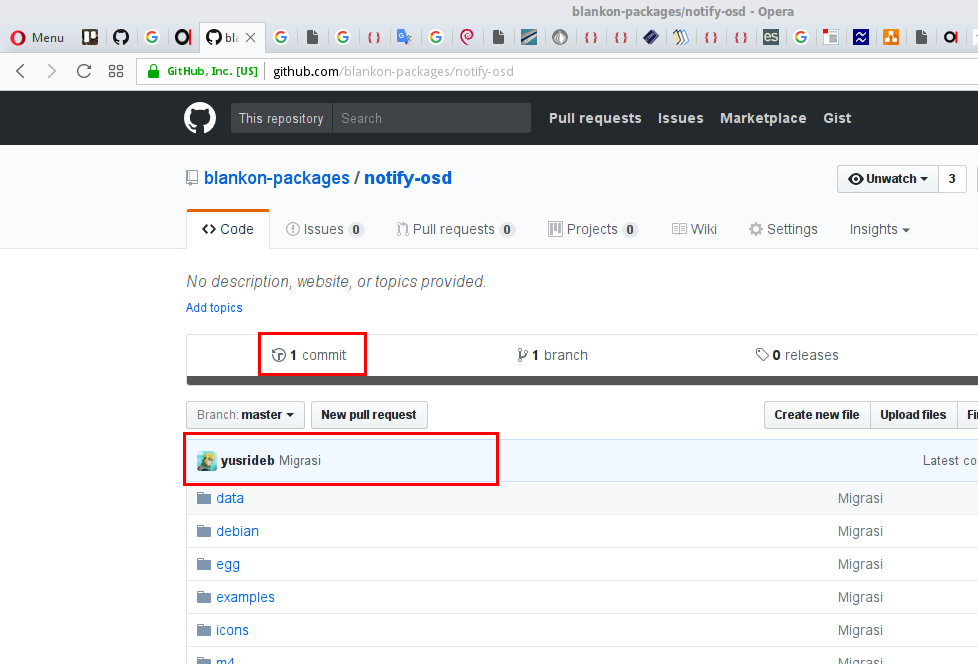
\includegraphics[width=12cm]{pkg-github-no-convert.png}
	\caption{Contoh paket yang diupload tanpa konversi format ke github}
	\label{fig:bab3_pkg-gihub-no-convert}
\end{figure}

\noindent
Untuk memperbaiki repositori ini, sebenarnya bisa langsung menghapus repositori di akun github, kemudian mengupload ulang paket yang sudah dikonversi ke format git. Jika hanya 1 paket mungkin tidak masalah, namun jika sudah terdapat repositori yang harus dihapus kemudian diupload ulang ke Github, maka beresiko salah hapus repositori. 

\noindent
Untuk melesaikan permasalahan seperti ini \textit{BlankOnDev Tools} menyediakan fitur untuk perbaikan repositori github yaitu dengan cara seperti yang ditunjukkan pada upabab \textit{\ref{sec:pre_impl_pros_mig}. Proses Migrasi Paket, bagian \ref{implm_4} dan bagian \ref{implm_5}}. berikut Ilustrasi penyelesaian masalah :

\subsection{Problem Solved dengan perintah \texttt{boidev bzr2git <cmd>}}
\label{sec:problem-solved1}
\noindent
Pada contoh ini nama paket yang bermasalah yaitu \textbf{notify-osd}, berikut daftar perintah yang digunakan untuk menyelesaikan masalah :
\begin{itemize}
	\item Perintah \texttt{boidev bzr2git branch \textbf{notify-osd}}
	\item Perintah \texttt{boidev bzr2git bzr-cgit \textbf{notify-osd}}
	\item Perintah \texttt{boidev bzr2git re-gitpush \textbf{notify-osd}}
	\item Perintah \texttt{boidev bzr2git git-check \textbf{notify-osd}}
\end{itemize}

\noindent
Rangkaian proses penggunaan perintah :

\begin{lstlisting}[language=ShellBash3]
$ boidev bzr2git branch notify-osd

Rilis Active : tambora

You want to Re-branch [y/n] : y

Bazaar re-branch for packages : "notify-osd"
Action re-branch for packages "notify-osd" 

======== Packages notify-osd has been finished to bzr branch ========

\end{lstlisting}

\begin{lstlisting}[language=ShellBash3]
$ boidev bzr2git bzr-cgit notify-osd

Rilis Active : tambora

Converting .... 


======== Packages notify-osd has been finished to convert ========

\end{lstlisting}

\begin{lstlisting}[language=ShellBash3]
$ boidev bzr2git re-gitpush notify-osd

Rilis Active : tambora

Re-push to GitHub .... 
----------------------------------------


Username for 'https://github.com': yusrideb
Password for 'https://yusrideb@github.com': 

re-push to git for packages "notify-osd" has success. 

\end{lstlisting}

\begin{lstlisting}[language=ShellBash3]
$ boidev bzr2git git-check notify-osd

Rilis Active : tambora
Check Repo [notify-osd] on github : repo_github = master, tambora 

git check repository for packages "notify-osd" | repo_github = master, tambora. 
\end{lstlisting}

\noindent
Hasil dari keempat perintah diatas yaitu :

\begin{figure}[H]
	\centering
	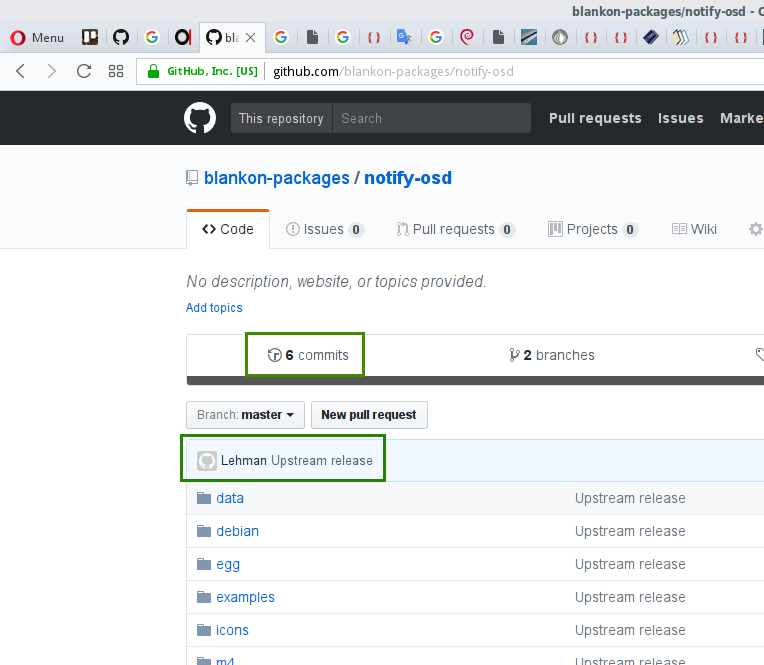
\includegraphics[width=95mm]{solved-github-no-convert.png}
	\caption{Penyelesaian masalah : Format paket belum dikonversi ke format git}
	\label{fig:bab3_solved1-gihub-no-convert}
\end{figure}

\pagebreak
\subsection{Problem Solved dengan perintah \texttt{boidev bzr2git}}}
\noindent
Pada bagian ini akan diilustrasi penyelesaian masalah mengunakan perintah \texttt{boidev bzr2git}. Berikut Ilustrasinya :


\begin{lstlisting}[language=ShellBash3]
yusrideb@pemaket:~$ boidev bzr2git

Rilis Active : tambora

---------------------------------------------------------------------------
Choose Action : 
---------------------------------------------------------------------------
1. All Packages
2. Specific Group Packages
3. Single Packages
Answer: 3

Enter packages name : notify-osd

Action re-branch for packages "notify-osd" 
[success] Action "bzr branch -> notify-osd" : 1
[success] Action "bzr convert git -> notify-osd" 1
[success] re-Action "bzr convert git -> notify-osd" 1
[success] Action "re-git push -> notify-osd" 
[success] Action "git check -> notify-osd" repo_github = master, tambora

========= Migration packages "notify-osd" has been finished =========
\end{lstlisting}

\noindent
Output Perintah :

\begin{figure}[H]
	\centering
	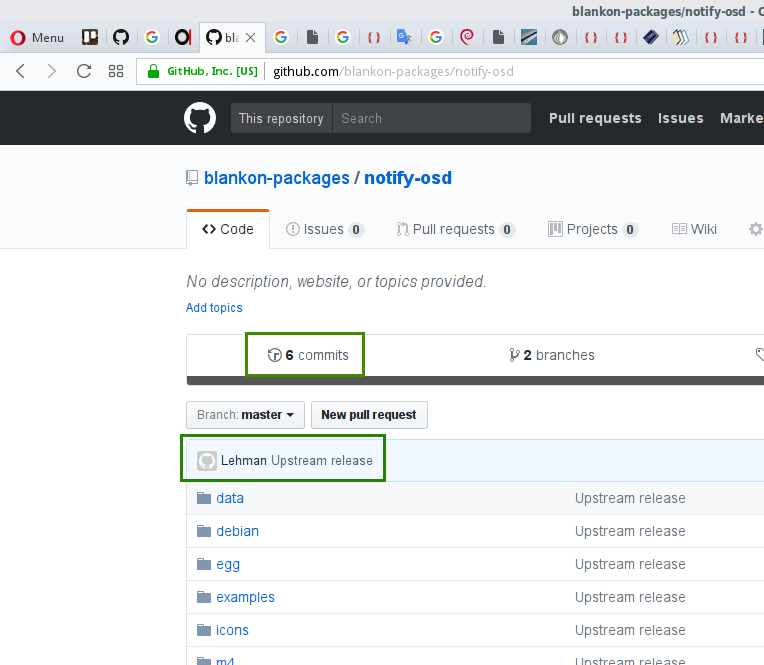
\includegraphics[width=95mm]{solved-github-no-convert.png}
	\caption{Penyelesaian masalah : Format paket belum dikonversi ke format git}
	\label{fig:bab3_solved2-gihub-no-convert}
\end{figure}

\section{Paket github hanya memiliki 1 jenis \textit{Branch}}
\label{sec:problem-solved2}
\noindent
Berikut contoh paket yang di dorong ke github, namun tidak dibuatkan branch ke rilis \textbf{tambora}, hanya branch \textbf{master} saja.

\begin{figure}[H]
	\centering
	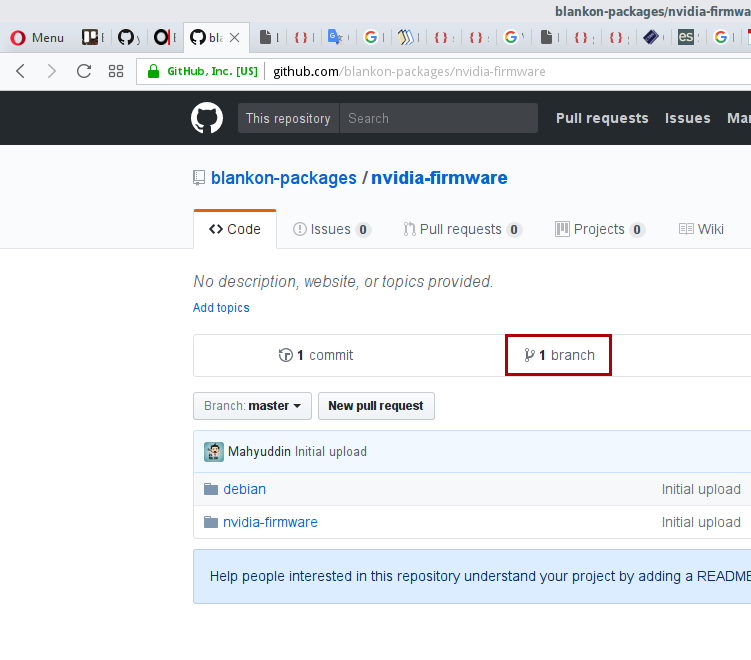
\includegraphics[width=8cm]{pkg-github-1-branch.png}
	\caption{Contoh paket yang diupload ke github, namun hanya memilik branch \textit{master}}
	\label{fig:bab3_github-1-branch}
\end{figure}

\noindent
Untuk memperbaiki repositori github seperti permasalah ini, dapat diselesaikan dengan seperti yang diilustrasi pada upabab \textit{\ref{sec:pkg-github-no-convert}}. Metode yang digunakan yaitu \hyperref[implm_4]{\textbf{Metode Split}} atau \hyperref[implm_5]{\textbf{Metode One-time}}. Pada bagian ini menggunakan \hyperref[implm_5]{\textbf{Metode One-time}}. Berikut ilustrasinya :

\begin{lstlisting}[language=ShellBash3]
$ boidev bzr2git

Rilis Active : tambora

---------------------------------------------------------------------------
Choose Action : 
---------------------------------------------------------------------------
1. All Packages
2. Specific Group Packages
3. Single Packages
Answer: 3

Enter packages name : nvidia-firmware

Action re-branch for packages "nvidia-firmware" 
[success] Action "bzr branch -> nvidia-firmware" : 1
[success] Action "bzr convert git -> nvidia-firmware" 1
Username for 'https://github.com': yusrideb
Password for 'https://yusrideb@github.com': 
[success] Action "git push -> nvidia-firmware" 1
[success] Action "git check -> nvidia-firmware" repo_github = master, tambora

=========== Migration packages "nvidia-firmware" has been finished ===========

\end{lstlisting}

\noindent
Hasil dari ilustrasi diatas :

\begin{figure}[H]
	\centering
	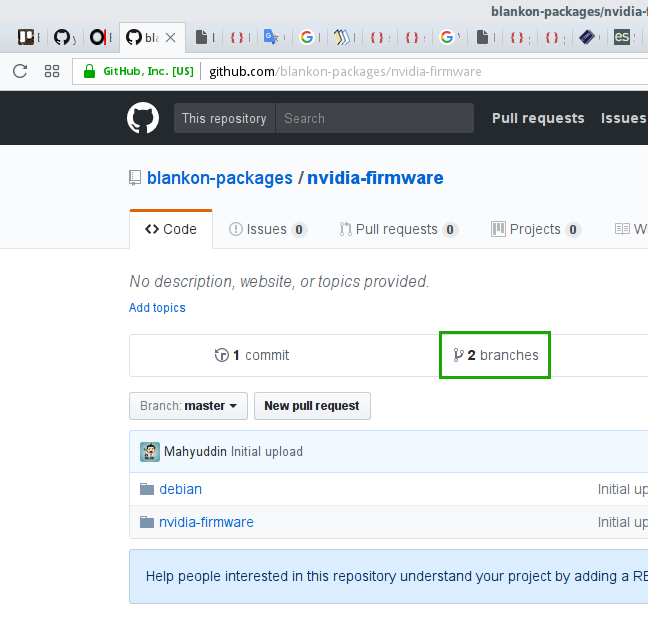
\includegraphics[width=10cm]{solved-github-1-branch.png}
	\caption{Penyelesaian Masalah : Repositori Github hanya memiliki type branch \textit{master}}
	\label{fig:bab3_solved-github-1-branch}
\end{figure}
	
	%% Appendix
	\appendix
\chapter{Appendix}

\section{Debian Manifesto}
\label{appdx::deb_manifesto}
\noindent
Yang ditulis oleh \textit{Ian A. Murdock} dan direvisi pada 1 Juni 1994.\\
Sumber :
{\scriptsize \url{https://www.debian.org/doc/manuals/project-history/ap-manifesto.en.html}}

\subsection{Apa itu Debian Linux ?}
Debian Linux adalah jenis distribusi linux yang baru. Daripada dikembangkan oleh satu individu atau grup yang terisolasi, seperti dstribusi Linux lainnya yang telah dikembangkan di masa lalu, Debian dikembangkan secara terbuka dengan semangat Linux dan GNU. Tujuan utama dari proyek Debian adalah untuk membuat distribusi yang sesuai dengan nama Linux. Debian sedang ditangani dengan hati-hatidan akan dipelihara dan didukung dengan perawatan serupa.

\noindent
ini juga merupakan usaha untuk menciptakan Distribusi nonkomersial yang dapat bersaing secara efektif di pasar komersial. Pada akhirnya akan didistribusikan oleh \textbf{The Free Software Foundation} dalam bentuk CD-ROM dan \textbf{The Debian Linux Association} akan menawarkan distribusi dalam bentuk Floppy disk (disket) dan Tape beserta panduan dalam format cetak, dukungan teknis dan kebutuhan pengguna lainnya. semua hal diatas hanya akan tersedia dengan hemat biaya, dan selebihnya akan diajukan untuk pengembangan \textit{Free Software} lebih lanjut untuk semua pengguna. Distribusi semacam ini sangat penting bagi keberhasilan sistem operasi Linux di pasar komersial, dan harus dilakukan oleh organisasi dalam posisi untuk keberhasilan sistem operasi linux kedepannya dan merekomendasikan perangkat lunak bebas tanpa adanya tekanan untuk mencari keuntungan lebih.

\subsection{Mengapa Debian dibangun ?}
Distribusi sangat penting untuk masa depan Linux. Intinya, dengan distribusi dapat memberikan kemudahan bagi pengguna yang sebelumnya mencari, mendownload, mengkompilasi, menginstal dan mengintegrasikan sejumlah tool penting yang cukup besar untuk merakit sistem Linux agar dapat bekerja dengan baik, kemudian diganti dengan menitikberatkan beban distribusi kepada konstruksi sistem yang akan ditempatkan pada pencipta distribusi yang karyanya dapat dibagi kepada ribuan pengguna dan hampir semua pengguna Linux dapat merasakan rasa pertama rilis Distribusi Linux dan sebagian besar pengguna akan terus menggunakan distribusi demi kenyamanan bahkan setelah mereka terbiasa dengan system operasi. Dengan demikian, distribusi memang memainkan peranan yang sangat penting.

\noindent
Meskipun sangat penting, distribusi hanya sedikit menarik perhatian pengembang. Ada alasan sederhana untuk ini yaitu "Pengembang tidak mudah dan tidak glamor untuk membangun dan membutuhkan banyak upaya terus-menerus dari sang pembuat untuk menjaga agar distribusi terbebas dari bug dan pembaruan". Ini adalah satu hal yang dapat dilakukan untuk membangun sistem dari nol. Ini cukup lain dari distribusi linux yang sudah ada sebelumnya, Ini dilakukan demi memastikan bahwa sistem mudah dipasang oleh orang lain, dapat diinstall dan dapat digunakan dengan berbagai konfigurasi perangkat keras yang berisi perangkat lunak yang bermanfaat bagi orang lain, dan diperbarui bila komponennya sudah harus diperbarui.

\noindent
Banyak distribusi yang telah dimulai sebagai sistem yang cukup baik, namun seiring berjalannya waktu untuk menjaga distribusi menjadi perhatian sekunder. Kasus dalam hal ini adalah seperti \textit{Softlanding Linux System} yang lebih dikenal dengan \textit{(SLS)}. Ini mungkin distribusi Linux yang paling banyak dikuasai namun dipelihara dengan cara yang buruk. Sayangnya, ini juga mungkin sangat populer. Hal ini, tanpa pertanyaan, distribusi yang menarik banyak perhatian dari "Distributor" Linux komersil yang telah muncul untuk memanfaatkan sistem operasi yang semakin populer.

\noindent
Ini memang kombinasi yang buruk, karena kebanyakan orang yang mendapatkan Linux dari "distributor" dan menerima distribusi Linux yang kacau dan tidak terpelihara dengan baik. Seolah-olah ini tidak cukup buruk, "Distributor" memiliki kecenderungan untuk mengiklankan fitur "produk" yang non-fungsional atau yang sangat tidak stabil dari produk mereka. Dengan fakta bahwa, pembeli tentu saja akan mengharapkan produk itu sesuai dengan iklannya dan kenyataan, dan banyak orang percaya bahwa ini adalah sistem operasi komersil (dan kecenderungan untuk tidak menyebut bahwa Linux itu Bebas atau Distribusi Linux tidak distribusikan di bawah GNU General Public License). Untuk melengkapi semua ini, "Distributor" mendapatkan cukup banyak keuntungan dari usaha mereka membeli iklan yang lebih besar disebagian besar majalah. Ini adalah contoh klasik dari perilaku yang tidak dapat diterima namun dihargai oleh mereka yang sama sekali tidak tahu yang lebih baik. Jelas sesuatu perlu dilakukan untuk memperbaiki situasi ini.

\subsection{Bagaimana cara Debian untuk mengakhiri masalah ini ?}
Proses pengembangan Debian dilakukan secara terbuka untuk memastikan bahwa sistem memiliki kualitas terbaik dan didasari oleh kebutuhan komunitas dan kebutuhan pengguna. Dengan melibatkan orang lain dari berbagai kemampuan dan latar belakang, Debian dapat dikembangkan secara modular. Komponennya berkualias tinggi karena mereka yang memiliki keahlian dibidang tertentu diberi kesempatan untuk membangun atau memelihara komponen secara individu yang terlibat dengan \textit{Debian} diwilayah tertentu. Dan juga melibatkan orang lain untuk mendapatkan saran berharga demi perbaikan system, yang kemudian menjadi rujukan untuk dimasukkan ke dalam distribusi yang sementara dalam proses pengambangan. Dengan demikian, distribusi dibuat berdasarkan kebutuhan dan keinginan pengguna daripada kebutuhan dan keinginan konstruktor. Sangat sulit bagi satu individu atau kelompok kecil untuk mengantisipasi kebutuhan dan keinginan ini tanpa mendapatkan masukan dari orang lain.

\end{document}